\hypersetup{pdfborder=0 0 0}
%\vspace{10\baselineskip}


%\selectlanguage{french}


\section{Resume français}

Partie a été rédigée en anglais dans l'éventualité d'une soumission prochaine en tant qu'article....


%\noindent\fbox{\noindent\begin{minipage}{1\textwidth}
%\noindent La maquette tri-dimensionnelle NH-HR est la maquette la mieux résolue sur l'horizontale (45 m) et la verticale (40 niveaux $\sigma$) implémentée dans le cadre du présent contrat.  De façon originale, cette maquette permet la simulation des "grandes structures turbulentes" \textit{(LES)}. Elle est pour cela basée sur le coeur non-hydrostatique et non-Boussinesq CROCO et met en oeuvre les schémas d'advection d'ordre supérieur et les schémas de diffusion turbulente isotropes disponibles dans CROCO, trois éléments essentiels et indispensables pour simuler numériquement à minima les instabilités primaires amorçant la cascade turbulente directe. Une comparaison détaillée de la dynamique à haute résolution avec celle simulée avec la maquette à plus basse résolution (NH-REF, section \ref{section3DNHREF}) montre que les processus de grande échelle sont représentés de façon comparable dans les deux maquettes. La simulation NH-HR permet en outre un raffinement du train d'ondes solitaires et surtout une représentation cohérente et explicite des instabilités de Kelvin-Helmholtz générées au voisinage du jet méditerranéen.
%\end{minipage}
%}


 %Comme discuté à plusieurs reprises dans le présent rapport, les différentes maquettes implémentées et exploitées dans le cadre du projet Gibraltar 16CR01 ne sont pas figées mais en constante évolution. Les évolutions en cours sont multiples:
 %\begin{itemize}
 %    \item Le code communautaire CROCO et son coeur numérique non-hydrostatique et non-Boussinesq CROCO-NBQ sont aménés à évoluer. De nouveaux schémas d'advection, de fermeture turbulente LES ou plus fondamentalement de couplage des modes numériques (associés au \textit{mode splitting}) sont en cours de développement et de test.
 %    \item La quête pour une plus grande efficacité du code a déjà permis des gains importants depuis la première implantation de l'algorithme non-hydrostatique, non-Boussinesq dans le code de recherche SNBQ. Elle se poursuit actuellement avec le portable du code sur des machines à structure dite hétérogène (CPU-GPU).
  %   \item En lien avec les futurs gains en efficacité de calcul, la maquette à haute résolution NH-HR est aussi amenée à évoluer vers plus de réalisme: les conséquences du forçage par la circulation générale et la marée étant correctement appréhendées, le forçage atmosphérique peut désormais être introduit. Le domaine simulé est de plus en cours d'extension, en particulier vers l'ouest.
% \end{itemize}
 
 %Le raffinement local de la circulation générale ouvre donc aussi des perspectives pour une meilleure représentation du "mélange" dans les modèles numériques de bassin. On peut en effet supposer que le mélange induit dans des régions telles que la région du ressaut hydraulique à Gibraltar sera plus facilement localisé et ainsi beaucoup mieux quantifié si l'on est capable de simuler explicitement les plus grandes structures turbulentes dans cette région. Leur modélisation implicite dans les simulations RANS réalisées jusqu'à présent repose en effet entièrement sur des schémas de fermeture turbulente représentant les conséquences des instabilités primaires. La simulation explicite d'une partie au moins de ces instabilités (les "structures turbulentes de grande échelle") permet une comparaison avec des observations directes ainsi qu'une analyse plus fine de leurs conséquences. \\
%Dans la région du détroit de Gibraltar toujours, nous disposons enfin avec la maquette NH-HR d'un outil d'étude de la formation du jet méditerranéen. Les mécanismes de génération du contenu en vorticité potentielle peuvent ainsi être étudiés à partir d'une maquette d'extension horizontale légèrement plus étendue. Une telle étude devrait permettre de mieux comprendre comment les différents mécanismes induisant un mélange notable peuvent modifier le contenu en vorticité potentielle de ce courant, bien en amont de la génération des instabilités baroclines auxquelles il est finalement soumis.\\

%Les simulations numériques et l'étude de la dynamique de fine échelle ont montré la nécessité d'une simulation des \textit{grandes structures turbulentes (LES)} dans la région du détroit de Gibraltar et dans la foulée l'adéquation du protocole original de modélisation basé sur le code CROCO. Les processus de fine échelle (ressauts hydrauliques, trains d'ondes solitaires, mécanisme de génération du jet méditerranéen, ondes de sillage, structures tourbillonnaires, instabilités primaires de Kelvin-Helmholtz...) ont pu être simulés explicitement. A notre connaissance, cette dynamique de \textit{fine échelle} n'a pas à ce jour fait l'objet d'observations in-situ dédiées dans la région du détroit. Une campagne d'observations permettrait d'évaluer précisément la pertinence de ce protocole de modélisation et des choix numériques. Elle ouvrirait aussi la porte à de nouveaux développements en mettant en évidence les limites du système actuel et permettrait finalement de préciser la localisation, la périodicité et l'amplitude des processus et autres mécanismes de fine échelle mis en évidence.

%La simulation de la région du détroit avec des maquettes de mieux en mieux résolues a permis de montrer qu'une résolution de l'ordre de quelques dizaines de mètres (45 m pour 40 niveaux verticaux "$\sigma$") était à minima nécessaire pour modéliser explicitement les instabilités de type Kelvin-Helmholtz dans la région du détroit. Ces instabilités dites primaires initient localement la cascade turbulente directe conduisant au mélange des masses d'eau atlantique et méditerranéenne.\\
%Le code CROCO et son coeur non-hydrostatique et non-Boussinesq ont ainsi été implémentés dans la région du détroit de Gibraltar (maquette NH-HR) afin de réaliser une simulation explicite des grandes structures turbulentes \textit{(LES)} dans la région du détroit. A notre connaissance, une telle simulation avec un code à surface libre explicite est une première.\\

%La maquette NH-HR a de surcroît permis de confirmer les résultats obtenus par Bordois (2015) et Bordois et al. (2016, 2017) à partir de sections verticales 2D: caractéristiques spatiales et temporelles de l'onde solitaire, génération de solitons mode 1 et mode 2, génération d'ondes topographiques... Plusieurs réflexions des ondes solitaires sur les côtes bordant le détroit ont de plus été mises en évidence et comparées aux observations disponibles dans la région. La dynamique du ressaut hydraulique a pu être précisée et le développement d'instabilités primaires de type Kelvin-Helmholtz a été confirmée à l'interface entre les eaux méditerranéenne et atlantique. La génération de tourbillons d'extension réduite au passage des solitons internes a été confirmée et le rôle déstructurant de ces tourbillons sur les trains de solitons est actuellement en cours d'étude.
%La qualité de la simulation des ondes et courants de marée dans cette région d'extension réduite et très active dynamiquement a été évaluée et des stratégies de simulation ont été proposées et implémentées pour améliorer la précision numérique des prévisions.\\


%La simulation des grandes structures turbulentes \textit{(LES)} de la région du détroit de Gibraltar ouvre des perspectives prometteuses pour l'étude de la cascade turbulente conduisant au mélange des masses d'eau. L'océan global est en effet connu pour n'abriter qu'un nombre vraisemblablement limité de régions présentant un mélange notable des masses d'eaux: régions peu-profondes localisées sur les plateaux continentaux ou dans les détroits, couches limites de fond et de surface abritant de violents cisaillements de courant, régions abritant sporadiquement des déferlements d'ondes de gravité ou des instabilités convectives... En dehors de ces "patchs" de mélange localisés dans l'espace et le temps, le mélange diapycnal dans la majeure partie de l'océan demeure faible (Munk et Wunsch, 1998). Cette double localisation des zones de mélange intense a plusieurs conséquences:
% \begin{itemize}
%        \item Le mélange diapycnal demeure difficile à quantifier et ses conséquences difficiles à évaluer: il est en effet intimement lié à des mécanismes de "fine échelle" mais il a des conséquences importantes sur les caractéristiques des masses d'eau et sur le maintien de la circulation à l'échelle globale.
%        \item Les observations directes du mélange et de la cascade turbulente directe dont il est une conséquence sont difficiles à réaliser, relativement récentes et restent très parcellaires.
%        \item La simulation directe du mélange diapycnal dans les modèles numériques est impossible et sa paramétrisation complexe.
% \end{itemize}
% La présente étude apporte ainsi plusieurs types de contributions pour progresser vers une meilleure connaissance du mélange diapycnal et de ses effets induits.\\




%-------------------------------------------------------------------------------------
\section{Review of general points about circulation at Gibraltar (intro/biblio)}

The Atlantic / Mediterranean exchange occuring in the Strait of Gibraltar has been explained summarily in previous part (2D). It consists in Med waters exiting the Strait at depth as what has been dubbed the 'Mediterranean outflow' while Atl waters use this pathway to enter the Mediterranean basin at the surface.

Those Atlantic waters that enter the Mediterannean at the Strait are the principal contribution to the Med inflowing water budget, with the average transport of Atl waters at Gib being of 1Sv. The net exchange itself is of the order of 0.1Sv (positive entry for med) and offsets the otherwise net evaporation occuring on the integrated surface of the Mediterranean basin (rough estimation volume that gets evaporated ??? faudrait voir évolution surface découverte med et si prend évaporation uniforme, combien de temps pour évaporer (1000an a vu cette valeur?)). The Med basin, being a semi-closed sea. This means that the Mediterranean waters exiting the Strait of Gibraltar are the result of the transformations of Atl waters.
More details are provided in this section on the characteristics of the Strait, the exchange and its variability and the processes that take place during it.



(Sommaire de cette partie.... Review some aspects...., variabilty of baroclinic exchange, focus on the high frequency which involves the several mechanisms that are studied in high resolution numerical simulation in next section)



%deep convection dans le bassin ouest de la Méditerranée s’effectue en 3 phases (Naranjo2014): le pérconditionnement (la densifictaion en circulant en Med ... 
%Critère convection profonde, regarde eaux densité >1029,10kg/m³ et le MLD (mixed-layer depth) où la diffusion vertciale >0,04m2/s (Naranjo2014)
%Taux de formation eaux denses (=eaux profondes ?) en Med trouve entre 0,3 et 6 Sv(Naranjo2014)…




\subsection{Circulation in neighbouring areas (Cadix and Alboran)}

(de Pascual-Collar ; NAjanro 2012 ; Sanchez Garrido 2013 ;Lorente 2019 ; garcia lafuente 2017)


\textit{Atlantic side}

The surface waters that end up entering the Strait are NACW and SAW(refs...bcp). They are carried by the Potrugal and Azores Current into Gib as part of the eastern branch of the north atlantic subtropical gyre(Barton 2001)

Below this surface circulation, can find in the Northern Atlantic the med outflow/the mediterranean watermass that was transported out of the Strait by the MEditerreanaen outflow. It first flows along the bathymetry in the Gulf of Cadix, sticking to north bathymetry due to Coriolis force on the rapid westward flowing waters. There it constitutes a system of veins that has been sampled ... (Gasser 2017). At the Cap St Vincent, flow north between bank,  baroclinic instabilies are shed out of the outflow as lenses of salty veins propagating soutward and dubbed 'meddies' for Mediterranean eddies, that can subsiste for 4 years(ref). The rest of the outflow spreads in the western part of the north atlantic basin as the MW water mass that can be found at 1000m depth and enhances salinity of NACW, with a branch also flowing north to join more directlt(Jia 2007;...). Through those two(three avec meddies?) processes contribute to salinification of waters before they go north to convection and join the global circulation (Jia 2007).

\textit{Mediterranean side}


Surafce waters exiting the Strait at the east enter the Alboran Sea as the Atlantic Jet (AJ). The ciruculation of the Alboran Sea is variable, witht the most common state having two anticyclonic gyre (Wag ans EAG), but not uncommon that only one of the two is present (Pinnardi). The WAG is the first structure encountered by the Atlantic Jet, it can either join its northern branch or contribute to the destabilisation of teh gyre itself, selon intensity of the jet.(Sanchez Garrido 2013; Lorente 2019) 

At depth, several mediterranean water masses enter the strait. In the Alboran Sea the three usually are identified are LIW (for Leventine Intermediate Water, formed in Rhodes gyres, Pinardi 2015) and WMDW(West MEditerranean Deep Water; formed in Golfe du lion during winter convection, Pinardi 2015), but also TDW (Thryenian Deep Water, entre els 2) (Millot). There is a south/north repatition of those watermasses, with TDW, LIW more abundant in northern part of Alboran sea, and WMDW flowing more in south part. As the depth from teh Alboran to the Strait decreases, it is more difficult for the deeper WMDW to enter the strait. Mechanisms that help would be important production of deep waters that elevate the level of WMDW(...). But it is was also shown that strength of the gyre correlates/will command the 'efficiency' of evacuaing wmdw (ventilation...)//facilitated entry of WMDW in the Strait (Najanro 2012) facilitates the water that cross the sill by bernouilli suction effect (Najanro 2012;Kinder and Parilla 1987) (cette deuxième phrase dans partie détroit...) 


\textit{Gen}

Whether look at inflowing Atl waters or outflowing Med waers (inflowing/ouflowing in regard to teh Med basin) (n fact, med outflow incorporated atl waters, and vice versa al inflow has med waters..., while the inflow and outflow retain some signature, they also incorporporate siganture of the other water masses of the exchange
L’atlantic inflow est constitué de SAW (eaux de surafce Atlantique), Naw (north-atlantic central water, signature plus importante en spring tide, petite devant les deux autres) et de MOW (med outflowing water) (Macias 2006)

outflow est composé d’eaux Med (LIW,WMDW, WIW) et d’eaux Atlantiques (Millot 2006?)
Outflow med incorpore aussi eau atl à cause mélange qui a lieu a CS...   

Those are the water masses brfore the exchange, however they are not the weter masses that are ... The exchange at the strait does not conserve the T,S characteristics. Hence processes occur in the Strait itself that transform this water masses, ie mixing occurs, need to understand processes in the Strait itself.

%%%%%%%%%%%%%%%%%%%%%%%%%%%%%%%%
\subsection{Campagnes d'observations et simulations numériques à Gibraltar/ Observatons and siulatons of processes in the Strait of Gibraltar(avant ou pares partie morpho...)}


First campaigns were aiming to quantify teh exchange and understand better the med budget, the most extensive is  . But also observations of solitons duig this campaign, with Farmer and Armi(...) explaining how the soitons are created by the interaction of te exchange and tidal forcing. The solitons that had been seen before, but with remote sensing more observations. Only surface signel, Ponctual in situ campaigns also use veloity and hydological arking of teh solitons. observed more and more with ... (Lacombe 1988) ((((As well as the impat of those sall eneretical processes on biological tracers. plus tard)))
The (arggggg periodicity of teh exchange s wel aknowledged, means that to have a budget need long term monitoring is more difficult, wat to survey the med budget , INGRES. also try to go beyond quantifying the budget and to connect more precisely the med outflow composition.
Moorings to monitor the med outflow and try to correlate its signature with events in the mediterranean (for exemple rate of formation of WMDW and other water masses). but due to vigorous mixing, med outflow difficult to single out all contributions.(garcia lafuente 2017) region of high trafic so long term mooring difficult especially in narrower sections. 1 mouillage Espartel sill longue durée (10 ans, Sammartino 2015, INGRES)

Many simulation experiments to understand propagation of solitons. As said in part. however only non-hydrostatic models can be used. The exchange as a part of the mediterranean and north atlantic circulation is more dfficult to represent as need big grids, . 
But the narrowness of the Gibraltar Strait means it is coarsely resolved in global (or even mediterranean) models. In global models parametrized...
Also studies to represent this exchange more explicitely, For exemple the model as local rafinemnt by putting Gibraltar in 'pole' position. ... also used imbrication model.

The characteristics of the Med waters that arrive at the eastern boundary of the strait are commanded by the processes of the med sea (convection, ...). 


In climate mode, parametrised with enhanced mixing (voir refdans Sanchez ronan 2018...)

(ref après dans les auters parties?)

Campagnes et obs in situ : Gibraltar 2008 (Bruno 2013) / INGRES (mooring à ES depuis 2004) / CANIGO( 95-98) Garcia Lafuente 2002 /Vargas 2006(moorings sortie est du détroit et CS) /2 mouillages mai 2003 propagation ISW (Sanchez Garrido 2008)/Watson 1990 obs radar gibraltar 3mois(mars-avril-juin) passage ISW (GEx)/Vasquez et al 2006\\

Tests simulation : Naranjo 2014, test modèle Med (avec imbrication?) avec ou sans la marée à Gibraltar / Soto-Navarro 2014 tests Med avec versions NEMO(coord z et eddy-permitting)



%%%%%%%%%%%%%%%%%%%%%%%%%%%%%%%%%%%%%%%%%%%%%%%%%%%%%%%%%%%%%%%%%%%%%%%%%%%%
\subsection{Morphologie et marée barotrope et masses d'eaux (et ajouter atm???)}
%%%%%%%%%%%%%%%%%%%%%%%%%%%%%%%%%%%%%%%%%%%%%%%%%%%%%%%%%%%%%%%%%%%%%%%%%%%%%
% \textit{\textbf{Why should we study this region ?}} \\

(Carte bathy ici?)

The Strait is inclined of 15° from the east. Camarinal Sill is the shallowest point with depth ranging from ... m to ... m(avg 300m). Relative to Camarinal Sill, Strait is narrower but deeper on the east side. On the west side, shallower, with two troughs, one shallow (...m) north and a deeper one (...m) south of a submarine relief called Majuan Bank. On the south side of which, another Sill, Espartel Sill. Those two troughs are the two pathways the MEd outflow take, with most of the flow taking the southern deeper path (18 \% au nord sleon Soto-Navarro 2014)



The barotropic M2 semi-durnal tide from the North Atlantic is the foremost signal, propatgating in the Strait from south to north with amplitude decreasing/halved from west to east. pronounced Neap-spring tide cycle.  Flood tide (courants barotropes vers Atlantique) // ebb tide (courants barotropes vers Méditerranée)(candela 1990? Sannino 2004?). Currents associated with the barotropic tide are same amplitude as the mean circulation...


A ES courant moyen mediterranean outflow : 0,15m/s(Sanchez Roman 2012). L’inflow atlantique presque tout le temps renversé à chaque période d e marée(Sanchez Roman 2012).

%(It was closed during Messinian, strong evaporation(sea level dropped by 1500m)that has left salt bed in Med, different hypothesis on how it opened again : tectonic activity (not local but away) lowers the area, fluvial erosion (lot of big drainage incision due to evaporation that took place (valleys of Rhone, Nile,etc.), raising of atl waters(but not likely, although pretty sure were some overflowing episodes)...(Loget, 2006)) 



%La PET (percentage of energy associated with tides) pour estimer importance de la marée dans courant total (Sanchez Roman 2012).

%%%%%%%%%%%%%%%%%%%%%%%%%%%%%%%%
%\subsection{Forçages atmosphériques}

%(Vents, variabilité, direction, puissance, effet sur les eaux, différence de pression Atl/Med) (upwelling)
%Effet du vent de surafce(peut aller 25m/s)à Gibraltar limité à une dizaine de mètres(Candela 1989). Ils sont cohérents avec presion Med et les ocurants en surafce.(viennent de quelle direction ?)

 Wind is funnelled through the strait and is either westward or eastward with speed can reach 25m/s(Candela 1989). Wind stress affects only the first tens of meters of circulation in the Strait (Candela 1989), which can be sufficient to affect the Atlantic Jet, either accelerating(and making it exit the Strait at various angle) or decelarting it(...). Otherwise, atmospheric forcing comes into play as integarted pressure over the Mediterranean bassin influence the net flow through the Strait(Garcia Lafuente 2002).



%Effet bromètre invers Atl/medd
%Effet gradient de pression Atl/med



%%%%%%%%%%%%%%%%%%%%%%%%%%%%%%%%
\subsection{Baroclinic Exchange variability}

The cirucilation of eastward Atlantic waters at the surface and westard Mediterranean waters at depth sets up a baroclinic exchange in the Strait of Gibraltar. Due to amplitude of teh barotropic currents, it is intermitent with regard to the M2 tide,can see it as average with tidal contrib as eddy-fluxes(Naranjo 2014, etc..)//  but is in average ... .  Can see other more long-term signal, with other components beside semi-dirunal tide following Candela 1991 (ou Vargas 2006) that are subinertial (from some days to some months) , and low frequency range (seasonal to interannual)

The lower frequency variability relates to tmospheric foricing


%(déjà dit dans 2D...
%Représentation dans le détroit : bicouche ou une troisième couche qui représente les eaux interfaciales (Sannino 2009, Bray et la 1995). Couche interfaciale finie à cause entrapinement et mélange entre les deux masses d'eau, à contribution à l’échange (Vargas2006). Approx bicouche reste valable (Vargas2006). Si prend bicouche : si le transport dans une couche n’est aps égal d’une section à l’autre du détroit, internal divergence/zone entre les deux peut srevir de réservoirs←cette inégalité vient d’une excursion de l’interaface accompagnée du transfert du signal de marée d’une couche à l’autre(Sanchez-Roman2012).
%Choix de l’interface : bicouche : Vargas 2006, prend isohaline qui maximise différence entre flot entre les deux couches // Sanchez-Roman 2012, niveau où à le maximal vertical shear of horizontal velocity

%Passive Layer / Couche passive, dans le bicouche, la couche qui…\\

Le détroit de Gibraltar fonctionne comme un estuaire inversé (SAnnino 2009, Naranjo2014,etc…) (parce que dans estaire couche du haut va vers l’océan alors qu’ici couche du haut rentre dans bassin?)
L’échange (moyen?) barocline à Gibraltar est forcé par la perte de flottabilité en Méditerranée (NAranjo2014). Il ets de l’rdre de 1Sv alors que l’échange net est de l’ordre de 0,1Sv (Vargas 2006). L’échange barocline a des variations qu’on sépare en 3 bandes de fréquences : tidal /subinertial (=de quelques jours à quelques mois) / low frequency (seasonal and interanual).
Il y a 4 composantes à l’écoulement à Gibraltar (selon Candela 1991) : forcé par la marée / forcé par les variations de pression atmosphériques en Med (effet baromètre inverse, force la surafce libre et donc le flot à travers Gibraltar)/ forcées oar le gardient de pression entre la Med et l’Atlantique / associé aux ISW\\



%(déjà présentation échange dans partie 2D... remets le bilan simplifié?)
%\textit{Two-conservation-equation model.}\\
%To study this exchange, a very simple steady-state model of the exchange at the strait of Gibraltar can be expressed with a system of two basic conservation equations :\\


%Mass conservation leads indeed to : 
%\begin{equation}  
%	\label{Eq_mass}
%    \displaystyle   
%  	Q_A+Q_M = E-P
%\end{equation}
%and conservation of salt requires: 
%\begin{equation}  
%    \label{Eq_salt}
%    \displaystyle   
%    Q_A S_A + Q_M S_M =  0
%\end{equation}
%where $Q_A$ is the volume flux of Atlantic water (positive value), $Q_M$ is the volume flux of Mediterranean water (negative value) and $E-P$ is the space-averaged Evaporation minus Precipitation (and river runoff) water budget over the whole Mediterranean Sea. $E-P$ is positive. $S_A$ ($S_M$) stands for Atlantic (Mediterranean) water mean salinity and $S_M-S_A\approx 2\mbox{\textperthousand}$ (Bethoux, 1979). The excess of evaporation corresponds to a yearly averaged loss of water of about 1 meter (Garrett et al., 1990).\\


%%%%%%%%%%%%%%%%%%%%%%%%%%%%%%%%
%\subsection{Variabilité de l'échange}

%(a plusieurs echelels de temps, quels mécanismes?)

%eddy fluxes are tidal contribution????(Naranjo 2014, etc..)



\subsubsection{Low Frequency variability}
(plutot faire des tirets ????)
Seasonal variability : 

Variabilité saisionière : En hiver, plus petite amplitude des couranst de marée mais subinertial flow augmente(SanchezRoman2012). En été inflow plus important, en janvier outflow plus important (Garcia Lafuente 2002). Interface moins profonde en début d’année, plus profonde en automne (approfondissement plsu lent que élévation) (GarciaLafuente2002).
A CS…




\subsubsection{Subinertial variability}
Fluctuations subnertielles contiennent 3 types(Vargas2006) : subinertiel barotrope (forcé par oscillations pression atmosphérique en Med) / subinertiel barocline (marée subinertielle (cycle vives-eaux mortes-eaux (Msf) et marée mensuelle (Mm))) /transort rectifié par la marée-flux turbulents (tidally rectified transport) (ou eddy-fluxes, la corrélation entre la profondeur de l’interface et les courants à la férquence de la marée). Les flux turbulents plus important à CS.
L’interface en neap tide au-dessus de Camarinal Sill est plus profonde et le shear est plus grand(de 20cm/s, car superposition long-term baroclinic exchange à un mode subinertielle barocline) et interface cross-slope est steaper(Vargas2006). Quand le transport net est vers la Med (ie max inflow) l’interafce est plus profonde que quand elle ets vers l’Atlantique




En spring tide, mélange plus intense (Naranjo 2014, Vargas 2006) (car augmentation de la turbulence Vargas2006)et le quasi-steady term est moins grand(Naranjo 2014), le sinstabilités de Kelvin-Helmotz sur l’ouest de CS et dans le bassinde Tanger augmentent l’aire de mélange(bassin de Tanger = réservoir d’eaux mélangées qui peuvent revenir en Med(entre autre par les IW qui font que AW est plus froide et +salée (ie, plus dense et moins de flottabilité, inetnsifie préconditionnement des eaux (?))) ou partir dans l’Atlantique nord)). Ce mélange diminue la flottabilité des eaux Atlantiques et impacte sa transition en intermediate/deep water, ie, les caractéristiques (l’hydrologie) des eaux Méditerranéennes (ie les eaux formées en Méditerranées) proviennent de leur perte de flottabilité lors de leur circulation en Méditerranée et des contraintes topographiques du détroit.



Le renouveau des eaux profondes en Méditerranée soulève les eaux profondes d’avant, qui peuvent se retrouver aspirer par le détroit de Gibraltar, la marée favorise al ventilation de WMDW(Naranjo 2014). On choisit comme critère pour les eaux profondes les eaux dont la température potentielle est <14°C(Naranjo2014).

Marée à Gibraltar refroidit les euax de la Mer d’Alboran (Naranjo 2014) , plus aurait effect advection de vorticité ?.. Voit transport cyclique par les ISW de chlorophylle vers l’est , fait des pulse (Bruno 2013)


\subsubsection{Tidal variability}
L’échange à Gibraltar à une composante eddy-fluxes qui augmentent l’échange à long terme (propprtion varie selon la scetion,(est plus garnde à Camarinal Sill (où le stermes d’eddy fluxes se manifestent lors de la perte du contrôle hydraulique))puis diminue des deux côtés, est 1\%) peut avoir 40\%(Naranjo2014)) et dont l’amplitude dépend du cyle vives-eaux mortes-eaux (Narajo 2014). pour de smoyennes temporelles >1T, Echange moyen = flux moyen(ie vélocité moyenne*profondeur interafce moyenne)+moyenne des flux turbulents (Naranjo 2014). En spring tide flu turbulents contre-balancés/en équilibre(?) par autres termes diminués par mélange intense.





%%%%%%%%%%%%%%%%%%%%%%%%%%%%%%%%%%%%%%%%%%%%
\subsubsection{La variabilité haute fréquence, mécanismes de petite échelle}
(Contrôle hydraulique (chemin des eaux dans le détroit…,Solitons)

Mixing associated with soliton expected to be remote in Alboran Sea; however, originates from the hydraulic control at CS and the hydraulic jump that can be observed there, and this feature could be responsible for a lot of mixing (GarciaLafuente2011?).

Billows were observed in \citet{WG94} , that grow downflow as they are advected by med waters westward. Their origin was theorised to be Kelvin-Helmoltz type instability of the flow in the lee of the hydraulic jump where high shear between accelerated med waters and almost stagnant atl waters.



\textit{Controle hydraulique}

Contrôles hydraulique dans le détroit de Gibralar (Sanino et al 2009, ...). Selon le nombre et la location des sections supercritique dans le détroit, régime maximal (ausi s, veut ire pas eu beaucoup demélange depis la ormation de LIW dit overmixed, ie delta S petit (Garrette Bormans Thomson 1990) si grand dlta (Reid 979 (trouver cette réf!) aurait réponse plus lente à stratif et forçage thermohalin e med et Atl))ou submaximal (ce régime serait plus sensible au changement dans lux air-mer (Garrett 1990) )de l'échange de masses d'eau à travers le détroit ( Sannino 2009,...) et lié au bilant E-P en Méditerranée. Sait aps dans quel régime est , est-ce que variabilité, etc... Garrtt 1990, légèremet submaximal en moyenne et passe de max à submax (dit en début d'année plutt max, mais pas sûr et rien variab interann/multi-décennale etc)

Farmi et Armer 1988 ont identifié 4 contrôles hydraulique : 2 permanents (ouest ES, TN) 2 épisodiques (ES et CS). || Sannino 2007 1permanent (nord TN), 1 épisodique (CS, quand perd le contrôle relâche bore) || Vargas 2006 le contrôle hydraulique à CS est permanent sauf à certains moment au cours spring tide ||Sanchez Roman 2012 , contrôle ES permanent (96%du temps) sauf quand ebb tide de splus importantes vives-eaux.
Un critère pour criticalité à TN : uand la couche Atlantique se détache de la côte nord, alors elle (la couche atlantique)est supercritique (Sannino 2009 , avant Bormans?) (analogie dans un évier, voit as la couche?????)
LEs méthodes pour identifir controle hydrauliue : nombre de Froude composite (FA?, 2 couches) // Pratt 2008 2D, nb arbitraire de couches //nb de Froude dans Vargas 2006



\textit{Hydraulic jump at camarinal sill and Solitons}
%La génération des ondes internes peut être réalisée par un modèle hydrostatique, leur évolution et leur propagation par contre est non-hydrostatique(Brandt 1996).

Hyd jump at CS intense mixing (Wesson andGregg;Lafuente...)

Ziegenbein (1970) obs with moorings, obs in september 1868 with three morrings aligned from the etsern eand of the strait. 

The first description of the generation of the large amplitude solitary waves of Gibraltar is from Farmer and Armi 1988(ou theorie avant...1985 based on obs at knight inslet and fact also hyd control, analogous case to knight inlet, , described more in paper 1988), they pinpoint their generation as the relaxation of the hydraulic jump at Camarinal Sill. This generation process can be achieved in numerical simulation by hydrostatic models but need non-hydrostatic one for propagation (Brandt 1996 et (Vlasenko 2009)).

Cross the 1h following max outflow (Vasquez 2006), between 1h before and after high water for Farmer and Armi 1988. Vasquez 2006 also obsereved a signal they attributed to teh crossing of a mode 2 wave (but mode 2 soliton possible???), they think that the bore gets decomposed since mode 1 and mode 2 wave speed different (so control greter on mode 2?)

(Watson and Robinson 1990 described it furthermore
When obsereved, ISW are generated at each tide excpet when westward current are not strong enough for hydraulic criticality at for neap tide (Watson and Robinson 1990, Garcia Lafuente 2000). 

En mortes-eaux, phénomène des boiling water au-dessus de Camarinal Sill, des high amplitude steady topographix internal waves (ondes de sillage?) inhibent la génération du bore(Bruno 2002).

(obs où)(Watson and Robinson 1990) In this same paper found temporal periodicity of 6 to 20 minutes, wavelength from 0.5 to 2.5 km, phase speead between 1 to 2m/s, amplitude up to 60m, up to 12 waves in a wave paclet. (??)
Caractéristiques de sISW diverses études (?) période de sondes entre 6 et 20 minutes / longueur d'onde entre 0.5 et 2.5 km / vitesse de phase entre 1 et 2 m/s / amplitude peak-to-trough jusqu'à 60m / jusqu'à 12 ondes par paquet (Watson and Robinson 1990). Watson and Robinson 1990 : entre 1 et 7 ondes par paquet/periode de 10à15min/longueur d'onde entre 0.5-2km/vitesse entre 0.4et2.5m/s
A la sortie est du détroit, le soliton est réfracté. Sa forme est soit une curbe régulière, soit avec un angle franc au nord (Watson and Robinson 1990).


Brnadt 1996, point out that on (sat or radar image ? two hydraulic jump..., 

%Le bore traverse au-dessus du seuil de Camarinal environ 1h avant la marée haute (entre 1h avant et 1h après)(Watson and Robinson 1990, vient Farmer Armi 1988).

(aussi papier obs avion??)


%Solitons observés à presque toute sle smarées sauf parfois en neap tide quand les courants d’ouest qui précèdent normalement dans le cycle de marée la propagation d’ISW sont pas assez fort pour qu’il y ait génération d’ondes internes au niveau de Camarinal (pas de flot supercritique)(Watson and Robinson 1990).

Image SAR/radar, image intensity augmente sur partie descendante internal wave et diminue sur partie montante
Observation radar de sISW : highest back-scattered signal proportonnel à la convergence des couranst de surafce(Izquierdo 2001).

Le bore/soliton arrive dans le détroit de Tarifa ntre 0,5et 4,5h aprs la mére haute (à Ceuta) et à l’entrée de la mer d’Albpran entre 5et 12h après la marée haute(SanchezGarrido 2008(mesures))(voir si concorde avec farmer and Armi).

Farmer and Armi gave a first approx of speed of propagation of the wave, however, 

Variability in the propagation speed due to the fact that in spring tide, barotropic current can be close to the interfacial propagation speed (especially at narrowest point of the strait, which also corresponds usually at when the tide is max eastward when the soliton is in the area(SanchezGarrido 2008)) of the wave itself (the wavespeed)(SanchezGarrido 2008), and since diurnal inequality is higher in spring tide can have important difference in two consecutives tidal cycle during spring tide, with hours of discrepency in the tidal cycle regarding the arrival time of the soliton at a certain point (ex. between 5h and 9h post high water at Gibraltar) (SanchezGarrido 2008  (uaais Watson et Robinson 1990). (This can be further reinforced by wind accelerating the surface atlantic layer...(???))
With morrings at TN and at long of CEuta, Sanchez Garrido 2008 find propagation speed between 1.2m/s and 2m/s, obs in may 2003.

On observational data, can see that the wave packet is usually desorganized, indeed phase speed is linked to the wave amplitude, which would mean that the packet's leading wave should be the one with gertest amplitude, the second with secondmost amplitude and son on, but oservations not this. (Vlasenko 2009 found was well organized 46.6\% of the time, they posit it could be becuse of the leading wave losing energy to interaction with lateral boudnaries or bottom refraction)


(Mot sur réflexion??? quel papier)

The solitons transport chlorophyll to the east, that is 'pumped' from coastal waters during hyd jump (separer assertion en 2, mettre dans partie hyd jump cobergence des eaux cotieres...) (Bruno 2013)


%Les courants de marée ont une vitesse comparable à la vitesse de propagation intrinsèque du bore, ce qui explique la variabilité dans la vitesse de propagation de sISW (SanchezGarrido 2008).


Le mélange à Camarinal Sill (et dans Bassind e Tanger), en vives-eaux malénge amène eaux profondes riches en nutriments dans Atlantic inflow(Macias 2006).

Le ressuat hydraulique à Camarinal Sill… En établissant le ressaut hydraulique à CS, aspire des eaux côtières riches en chlorophylle au centre du détroit (Bruno 2013).

Les LAIWS générées à Camarinal y restent environ 4h avantd epouvoir se propager (Vlasenko 2009).

On observe deux ressauts à camarinal (Brandt 1996).

%L’inégalité diurne est importante et responsable pour une différence de vitesse de propagation entre deux bores consécutifs de (environ?jusqu’à?)0,7m/s (SanchezGarrido 2008). L’inégalité diurne est plus importante en période de vives-eaux(SanchezGarrido 2008). Dans l’est du détroit, les courants dans la cuche atlantique ont une forte composante diurne, deux paquets consécutifs d’ISW arrivent à la sortie est du détroit pas au même moment dans le cycle de marée (ex au niveau de Gibraltar entre 4 et 9h après la marée haute), quan dle courant dan la couche Atlantique ets plus fort, le ssolitons arrivent plus vites(Watson and Robinson 1990). Inégalité dirune est plus garnde en neap tide (ou à cette période de mesure spring tide correspondait cycle qui commande diurne ???)(Watson and Robinson 1990).

%La vitesse maximale du bore est atteindte dans TarifaNarrows (détroit de Tarifa), car à ce moment là est en max inflow (SanchezGarrido 2008). C’est aussi là que les courants de la couche Atlantique sont les plus forts car la cross-section y ets minimale (Watson and Robinson 1990).



%Les ISW sonts générées au seuil de Camarinal. 2 types d’ondes internes sont générées, mode 1 et mode 2(Vasquez 2006).

%Le bore barocline transite vers l’est au-dessus du seuil de Camarinal 1h après l’outflow maximum (Vasquez 2006).

%Pendant l’outflow le sondes internes sont coincées sur le flanc ouest du seuil de Camarinal et se décomposent. Lorsque la marée change de sens le mode 1 est libéré puis le mode 2(Vasquez 2006).

%Les LAIWS (large amplitude internal solitary waves) obsérvés dans le détroit de Gibraltar proviennent de l’évolution non-linéaire du bore généré au-dessus du seuil de Camarinal (Vlasenko 2009).

Le bore génère des ondes secondaires en se propageant dans le détroit. Une partie de cette dispersion est du à la rotation de la Terre (Vlasenko 2009).

%Normalement un paquet de soliton se propage de façon ordonné (celui qui a la plus grande amplitude s epropage plus vite), mais en sortie du détroit de Gibraltar (à l’est de Gibraltar et ceuta, dans la mer d’alboran) on ne les observe que 46,5 \% du temps, le reste est désordonnés (Vlasenko 2009).  Vlasenko 2009 : serait à cause réfraction sur la géométrie du fond(?) ou de sinétractions avec le sbords latéreux(?)(la première odne perd de l’énergie qui ets absorbée par la suite du train ?).








%-------------------------------------------------------------------------------------
\section{Simulation VHR and Local ocean dynamic/processes in the Strait}

After the 2D study of Hilt 2020 seeing the improvement of non-hydrostatic and decadal resolution, it was applied to 3D simulatin of the flow. This section discribes the configuration of this simulation and give an overview how the local fine scale tidal processes discribed in the previous section are represented there and more importantly how they are diagnosed in this numerical framework. The next section afterward will focus on the more local process of the crossing by mediterranean waters of Camarinal Sill.



\subsection{Numerical Configuration}
\subsubsection{Numerical framework}

Use CROCO-NBQ as was the case in Hilt 2020 (see a presentation of CROCO-NBQ there ) . The table ..., 

40 sigma level homogeneously distributed in the water column, in the area of the Sill sufficient to be more resolved on the vertical than in horizontal direction (see table).

%Domain area 6°4.8'W  5°3.4'W;35°23.8'N  36°27.4'N 

Bathymetry data from SHOM (MNT100(toujour sle cas???)), smoothed for pressure gradient...

Initialisation and open boundary conditions are from a simulation of the operational Med and Black Sea ENEA using MitGCM (ENEA, Rome)\footnote{http://www.enea.it/it/seguici/pubblicazioni/pdf-volumi/cresco-report-2016.pdf}, whch serves as parent simulation. interpolated on sigma grid, integrates tidal forcing. No atm forcing/surface flux. 

First 6 hours of simulation are run in CROCO-Hydro at 50m resolution and the last field is used to restart in NBQ mode. Otherwise the balance in MitGCM (dx $\approx$ 700m in the Strait) is to coarse for stability at 50m.

Non-linear equation of state

Either Smagorinski closure scheme or GLS k-$\epsilon$ in part, only Smagorinsky in part.. .



\begin{table}[!h]
        %\begin{minipage}{.6\textwidth}
        \centering
        \begin{tabular}{|p{\linewidth/3}|c|c|}
                \hline
                %Coeur numérique & \multicolumn{2}{c|} {CROCO-NBQ} \\
                Grid Extension & \multicolumn{2}{c|} {6°4.8'W  5°3.4'W ;}\\
                & \multicolumn{2}{c|} {35°23.8'N  36°27.4'N}\\
                Number of horizontal grid points & \multicolumn{2}{c|} {2049x2621}  \\
                Number of vertical $\sigma$-levels & \multicolumn{2}{c|} {40} \\
%                %\hline
                $\Delta x = \Delta y$ & \multicolumn{2}{c|} {45 m}\\
%                %\hline
                Depth & Min & Max\\
                & 26 m & 960 m\\
                $\Delta$z & 0.7 m & 24 m\\
                %Nombre de coeurs & \multicolumn{2}{c|} {447 (+1 serveur xios)}\\
                Internal time-step ($\Delta t_s$) & \multicolumn{2}{c|} {1 s}\\
                External time-step ($\Delta t_f$) & \multicolumn{2}{c|} {1/11 s(change 1/14)}\\
                Advection scheme & \multicolumn{2}{c|} {WENO-5} \\
                Viscosity $\nu$ & \multicolumn{2}{c|} {10$^{-6}$ m$^2$/s} \\
                Diffusivity $K_\rho$(aussi Ks et Kt) & \multicolumn{2}{c|} {10$^{-6}$ m$^2$/s}\\
                Pressure/accoustic wave speed$C_s$ & \multicolumn{2}{c|} {400 m/s}\\
                Tidal harmonics (from ENEA) & \multicolumn{2}{c|} { $\text{M}_{\text{2}}$, $\text{S}_{\text{2}}$,$\text{K}_{\text{1}}$, $\text{O}_{\text{1}}$ }\\
                \hline
        \end{tabular}
        \captionof{table}{.....}
        \label{tab_NH-HR}
        %\end{minipage}
\end{table}


%L'hydrologie, les courants de marée et la circulation générale sont forcés comme pour la maquette NH-REF à partir d'une simulation hydrostatique "Mère" MitGcm du modèle opérationnel de la Méditerranée et de la Mer Noir de l'ENEA, gracieusement fournie par l'équipe de G. Sannino (ENEA, Rome)\footnote{http://www.enea.it/it/seguici/pubblicazioni/pdf-volumi/cresco-report-2016.pdf}. Ce forçage est utilisé comme condition initiale et comme conditions aux frontières ouvertes. Cette simulation "Mère" a une résolution horizontale variable d'environ 700 m dans la région du détroit, soit environ une quinzaine de fois supérieure à celle de la maquette à haute résolution NH-HR. Ce saut en résolution relativement élevé est associé à un changement de coordonnées verticales (le MitGcm est basé sur une grille à niveaux z, CROCO sur une grille $\sigma$).  Les cœurs dynamiques utilisés dans les simulations Mère et NH-HR sont de plus différents: la maquette NH-HR est en effet non-hydrostatique et non-Boussinesq alors que la version du modèle MitGcm utilisée pour réaliser la simulation "Mère" est hydrostatique et Boussinesq.\\
%L'ensemble de ces différences est à l'origine d'un choc violent lorsque la simulation NH-HR est initialisée et forcée directement à partir de la simulation Mère MitGcm. Un tel choc entraîne une période de \textit{spin-up} de plusieurs heures durant lesquelles la qualité des caractéristiques des masses d'eaux méditerranéenne et atlantique est peut-être fortement dégradée. En conséquence, un protocole de simulation spécifique a été mis en place:
%\begin{itemize}
%        \item La simulation à haute résolution (HR) est initialisée et forcée par la simulation Mère MitGcm.
%        \item Durant les 6 premières heures de simulation, le coeur hydrostatique, Boussinesq de CROCO est implémenté, limitant ainsi le choc initial et permettant une première mise en équilibre des champs initiaux sur la bathymétrie à haute résolution.
%        \item La simulation HR est alors redémarrée (\textit{Hot Restart}) en version non-Hydrostatique et non-Boussinesq.
%\end{itemize}
%Quatre ondes de marées sont forcées aux frontières latérales: ($\text{M}_{\text{2}}$, $\text{S}_{\text{2}}$, $\text{K}_{\text{1}}$, $\text{O}_{\text{1}}$). Ce forçage est intégré dans les sorties issues de la simulation MitGcm à 700 m.\\


\subsubsection{Tidal forcing and simulation period}
Tidal forcing is integrated to the boundary forcing by the parent simulation. It comprises four harmonics (?)($\text{M}_{\text{2}}$, $\text{S}_{\text{2}}$, $\text{K}_{\text{1}}$, $\text{O}_{\text{1}}$)

In september are greatest(?) tidal coefficients, link to equinox.

Three different periods are investigated among neap tide spring tide cycle, the date of the beginning and end of each NBQ simulation is surmrised in table \ref{tab_dates_MIV}, and does not include the 6hour hyrostatic spin up period. The comparison between tidal gauge at Tarifa is in figure 

\begin{table}[h]
        %\begin{minipage}{.6\textwidth}
        \centering
        \begin{tabular}{|c|c|}
                \hline
                Situation & Dates (UTC)\\
                \hline
                Marées Moyenne (MM) & 10/09/2017 19h00 - 13/09/17 01h00  \\
                Mortes Eaux (VE) & 13/09/2017 16h00 - 15/09/17 17h00 \\
                %\hline
                Vives Eaux (ME) & 19/09/2017 22h00 - 21/09/17 23h00  \\
                \hline
        \end{tabular}
        \captionof{table}{Périodes de simulation pour les 3 sitituations VE, MM et ME (format date JJ/MM/YY????)}
        \label{tab_dates_MIV}
        %\end{minipage}
\end{table}

Figure... compare the sea level anomaly at the closest grid point to Tarifa (coord -5.6° - 36.01°) in both the VHR simulation and the parent MitGCM simulation, and compares it to Tarifa's tidal gauge data made available by spanish institute \textit{Puertos del Estado} (Mettre une ref pour data...). 'Dephasage' is under one hour when it is , the most 'dephase' is for the lowest amplitude tidal period during neap tide, retains the lower amplitude of anomaly of MitGCM (around 10 cm), that can be explained by difference in bathymetry in simulation at proximity of near the coast, the lack of more tidal harmonics, lack of atmosphere forcing.

%(Refaire figure en ajoutant ubar a camarinal sill en notant heures des max d'outflow...???)



%\begin{table}[h]
%        %\begin{minipage}{.6\textwidth}
%        \centering
%        \begin{tabular}{|c|c|c|c|c|}
%                \hline
%                Situation & \multicolumn{2}{c|}{Tarifa} &\multicolumn{2}{c|} {Ceuta}\\
%                &CROCO &MitGCM&CROCO &MitGCM\\
%                \hline
%                Mortes Eaux (VE) &10 cm &7 cm &9 cm& 6 cm\\
%                %\hline
%                Marée Moyenne (MM) & 13 cm&10 cm &12 cm&9 cm \\
%                Vives Eaux (ME) & 14 cm& 11 cm& 12 cm&9 cm \\
%                \hline
%        \end{tabular}
%        \captionof{table}{Erreur standard(rmse) de l'anomalie de niveau de la mer entre les simulations et les marégraphes. A REFAIRE? (IE pas bon sûr)}
%        \label{tab_dates_MIV}
%        %\end{minipage}
%\end{table}


\begin{figure}[!h]
        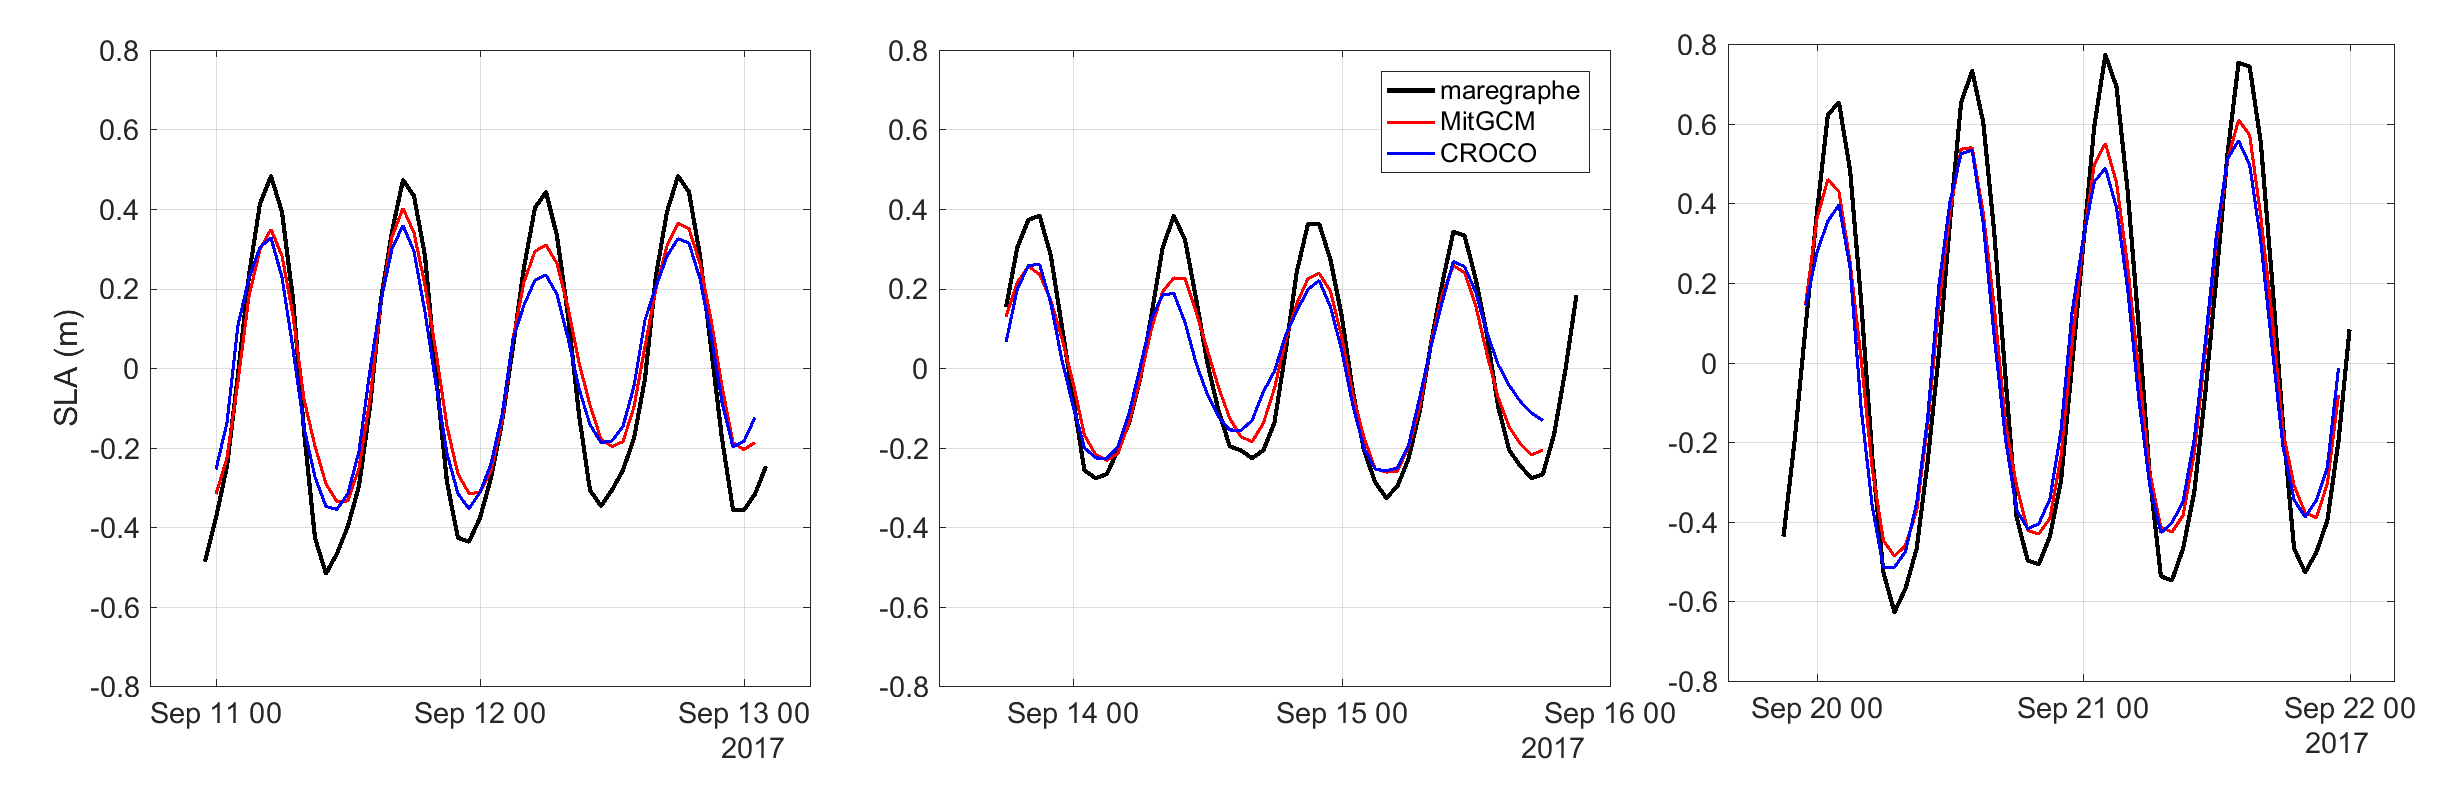
\includegraphics[width=\textwidth]{./GBR3D/SLA_Tarifa_ME2VE2IES.png}
        \caption{Anomalie du niveau de la mer (m) à Tarifa (36°N 5°36'W) enregistrée par le marégraphe  (courbe noire),
        interpolée dans le champ de forçage (courbe rouge), dans CROCO (courbe bleu) dans la situation ME (a), MM (b) et VE (c).
        En tirets bleus le signal filtré à 25h dans CROCO.}
        \label{fig_maree_tar}
\end{figure}

\subsubsection{Water masses}


\begin{figure}[!h]
        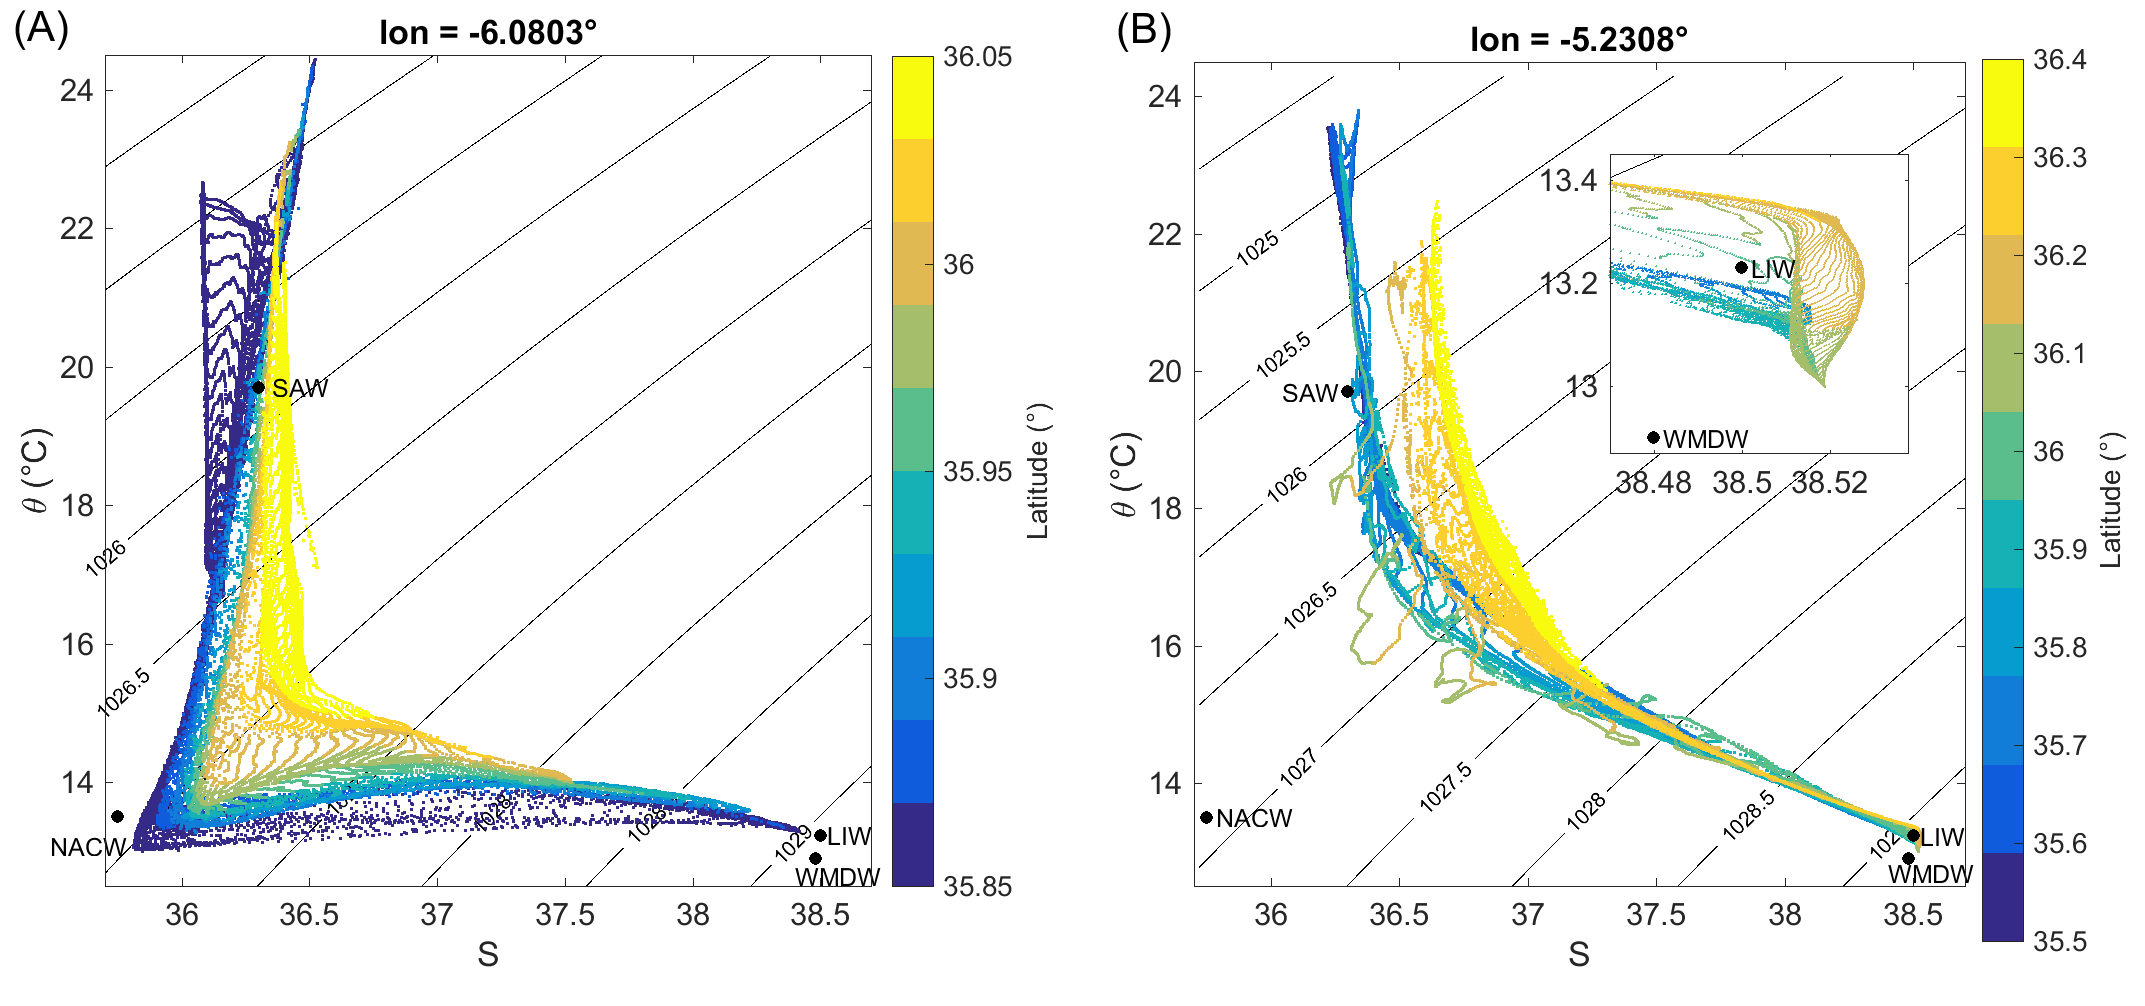
\includegraphics[width=\textwidth]{./GBR3D/WM_ini_IES.png}
        \caption{}
\end{figure}


Figure shows the T,S diagrams for east west entry of the Strait in initial tracer field of simulation Intermediate Tide. As expected, for med waters see on the west side two signals for the two pathways, on the east side see distinctly a deep water mass and an intermediate one (not the value found in biblio) that could be interpreted as WMDW and LIW, with the latter being present mostly on the northern part, difficult to say if other water masses. For atl waters, NACW present on west of domain, less on east. On east, see difference surface water north/south.

%In simulation, profile T,S are similar in their overall shape to what is bibliographycally expected, see mediterranean water masses distinct in latitude west of the sill.
%Although the water mass signature have some bias compared to existing observational data so they are to be adressed as generic mediterranean water masses, with the densest analogous to WMDW, if we distinguish two others east of the sill that may be analogous to LIW and TDW, those analogous water masses are denotes A,B,C centroid are taken from WM present east of the sill, but looking at water masses west of the sill they will simply be called OA and OB for med outflow water A and B. OA and OB are not differentiated by hydrological characteristics but simplt by latitude (ie the path taken along the strait).
%Mixing does not occur homogeneously along the strait and results in at least two distinctive enough med vein in the strait of Gibraltar. Furthermore, simulation permits to see variability in time is those two veins T,S characteristics at a given section, so the water mass being transported varies in time at the M2 time scale.




\subsection{Numerical diagnostics}
Mettre que définitions des diagnostiques, dans partie d'après y fait référence

\subsubsection{Interface definition}

Take a two-layer approach to the dynamic and definition of atl and med layer.

Following (Sannino?), the central salinity value of the interface is taken as the middle of the slope area in a hyperbolic tangent fit of the salinity profile at one grid point. This has been repeated for some ... accross the three simulations and along the Strait, can see that the pycnoncline is saltier east of the camarinal Sill. To define med and atlantic layer then chose a salinity of interface as a fuction of longitude :

\begin{equation}
	S_i(x)=tanh(\frac{x-X_{CS}}{DX})\frac{S_M-S_m}{2}+\frac{S_M+S_m}{2}
\end{equation}
with $X_{CS}=5.75^o$, $dx=0.25^o$, the location and width of the Camarinal Sill in degrees, $S_M=37.39$ and $S_m=37.1$ the max and minimum values

%This may not give the perfect interface at any given time...

\subsubsection{Froude layer number}

With de definition of the interface of paragraph. Can define a froude layer number. 

\begin{equation}
G^2=F_1^2+F_2^2 \ \ , \ \text{with} \ F_i=\frac{u_i^2}{g'h_i} , \ \text{with} g'=g \frac{\rho_2-\rho_1}{\rho_0}
\end{equation}

where $\rho_i$ averaged density in layer i,  u is averaged velocity norm (u and v) over the layer i of height h. If $F_i>1$ say that layer i is supercritical.


\subsubsection{Hydraulic Jump detection, acceleration of flow}
Given geometry of the strait can say that condition of conservation of flux through the area of the hydraulic jump. 
%Solution for hyd jump, when authors try to find analytical solution of hyd jump (biblio). Here not trying to find general approach but just a diagnosisi for Camarinal Sill. 
Detection based on the modification of the flow downstream of hydraulic jump. No trying to find analytical form of the hydraulic jump, only the consequence that the presence of hydraulic jump has on the flow.

\begin{figure}[!h]
 \centering
 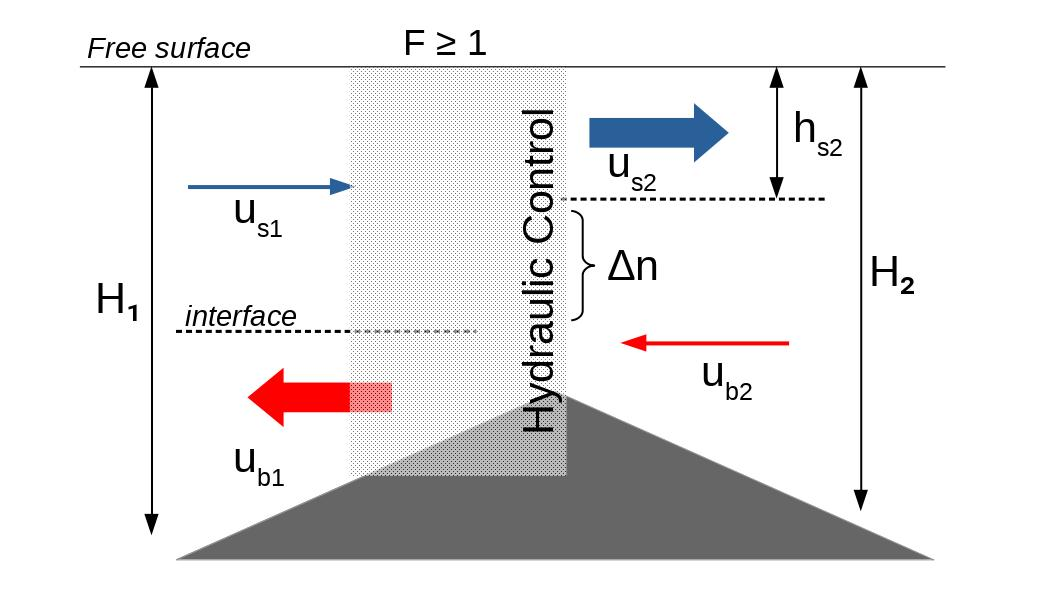
\includegraphics[width=0.5\textwidth]{./GBR3D/schema_diagressaut.jpg}
 \caption {Schematic of flow upstrean and downstream of hydraulic jump at Camarinal Sill, Strait of Gibraltar}
  \label{schemaRH}
\end{figure}


Assume that homongeneous flow in both atlantic and mediterranean layer (defined in regard to salinty as previously). Consequence of hydralic jump : pycnocnline depth varies greatly on short interval (non linearity?). Due to the geometry of the Strait, how the flow of Med water is constrained by bathymeetry, it is commanded by flow conservation, less so for Atlantic water that can disperse in part in upper layer on continental shelf. For lower layer This give us equation :

\begin{equation}
u_1 (H_1-b_1) = u_2 (H_2-b_2) 
u_1 (H_1-b_1)= u_1 (\Delta H + \Delta n) + u_1 (H_1-b_1) + \Delta u_b (H_2-b_2) 
\Delta u_b = -u_1 \frac{\Delta H + \Delta n}{H_2-b_2}
\end{equation}

To complete, can use another condition, the fact that in area oh hydraulic jump flow is critical, ie Froude number $\geq$ 1. We search minimal condition for hydraulic jump so $F=1$ or $U=c$ flow equal propagation/phase speed of internal wave, if we take the interfacial speed : 
\begin{equation}
|u_1|=c=\sqrt{g' \frac{(H_1-\Delta n - b_2)(\Delta n + b_2)}{H_1}}
\end{equation}



In the end, some parameters are chosen as threshold, the minimum excursion of the jump $\Delta n$ and the height of the Atl layer , and the reduced gravity

\subsubsection{Q parameter and derivated diagnosis}

To detect vortex structures without a proiori choosing a rotation axe as with vorticity diagnosis, can use parameter Q (refs)

\begin{equation}
Q=-\frac{1}{2} \frac{\partial u_i}{\partial x_j} \frac{\partial u_j}{\partial x_i} = \frac{1}{2} (\Omega_{ij}\Omega_{ij} - S_{ij} S_{ij})
\end{equation}
with $u_i$ the component of velocity, and $S_{ij}$ and $\Omega_{ij}$ are respectively symetrical and anti-symetrical parts of velocity gradient (comme ça se dit en anglais????). When $Q>0$, anti-symetrical term contribution, which denotes rotation, is predominent over the symmetrical, shear, part. ((It can also be viewed as a generalisation of Okubo-Weiss parameter used in 2D, however rotation is indicated by negative values for OW, but by positive values for Q parameter.))

Due to this advection, there are grid cells for which a succession of billows propagate. The temporal evolution of Q over such grid cell will show oscillations between high positive value (center of a billow/vortex) and low negative values (shear between two consecutive billows). This would mean a high value of standard deviation of this timeserie, as defined in equation \ref{eqstdQ} where the overbar denotes temporal average over 30 minutes, a period over which there will be minimal modification of the general flow in the Strait.

\begin{equation} 
\label{eqstdQ} 
    std ( Q ) (\vec{x},t)=  \sqrt{   \overline{Q (\vec{x},t)^{2}} -  \overline{Q(\vec{x},t)}^{2}       }
\end{equation}

By implementing this calculation directly in the code, we can asses where instabilities/vortexes propagate without having to make a huge volume of simulation outputs over the whole domain, those economising in storage place and data readability. Thus it is possible to create a map of standard deviation of Q which will reflect areas where KH billows will propagate in the simulation.


Standard deviation of parameter Q is computed as in \ref{eqstdQ} and for each 30 minute average interval the maximum standard deviation in the water column is outputed for each horizontal grid point. Figure \ref{fig3} shows this map for t=...H during outflow/rising water/... .

One can also use SVD of parameter Q, where as in SVD of Okubo-Weiss parameter in 2D chapter / case, complex SVD means see propagation in the left  term of temporal evolution... However thhis calculation is offline and necessitates a high frequency 3D output to pick up the relevent structures.


\subsubsection{Matching Pursuit}



Solutions of solitons are generally given by solution of KdV equation as the general form 
\begin{equation}
\eta(x,t) = A sech^2\bigg( \frac{x-Ct}{l} \bigg) 
\end{equation}
with A amplitude, C the phase speed and l a lengthscale. Those three parameters(?) are linked, and knowing two of them gives the third, for exemple greater the phase speed, greater the amplitude. Analytical expressions of those two remaining parameters varies on the choices made to solve the KdV equation and have in their expressions startification, etc. depth. 

Here chose solution for ... 


Locating ISWs in temporal signal of tracer in the water column (and in u? essayer) use Matching Pursuit algorithm. Rely on finding better convolution for the signal among elements of a 'dictionary' called 'atoms'. The shape of this atoms is decided by the user, here we chose Morlet waves, Dirac peaks, and define a 'soliton shape' from the analytical solution of the KdV problem. Additionally, the signal chosed as the basis for the Matching Pursuit will not be directly the depth of an isopycnal $\eta$ for it varies greatly due to internal tide but the trend $\partial \eta/\partial t$ for which at $x=0$ the expression derived from eq ... is :
\begin{equation}
\frac{\partial \eta}{\partial t} = \frac{2 C A}{l} \frac{sinh(-Ct/l)}{cosh^3(-Ct/l)}
\end{equation}

However, in this case the propagation speed of the wave is not only its phase speed, as it is advected by the currents, so $C=C_s+u$ with u the ambiant barotropic current.


%\noindent\textit{Repérer le passage de train d'ondes solitaires : Matching Pursuit}\\
%Une forme analytique de la perturbation de l'interface où se propage un soliton dans un fluide bicouche est donnée sous la forme : (general KdV formulation for one solitary wave in sech squared, two 'parameters'/'degrees', with amplitude linked to phase speed and wavelength, the latter have expressions depending on variables such as stratification and depth) However in a temporal serie the wave is also advected by , and it is this composite speed that defines the signal's form. take as parameters, depth, amplitude and speed, derivate from the couple depth/amplitude a first wavelength, it is compared to 
\begin{equation}
\eta = A sech^2\bigg( \frac{x-Ct}{l} \bigg) \ \ , \ \text{avec} \ l = \frac{2h_1h_2}{\sqrt{3A(h_1-h_2)}} \ \text{et} \ C=c_0 \ (1 + \frac{A}{2} \frac{h_1-h_2}{h_1h_2})
\end{equation}
où $\eta$ est la position de la surface isopycnale séparant les deux fluides, $h_1$ et $h_2$ sont les épaisseurs des deux couches de fluide de masse volumique $\rho_1$ et $\rho_2$ et $c_0=\sqrt{g'H}$ est la vitesse d'une onde longue interfaciale.
Pour localiser le passage de solitons dans un signal temporel de la colonne d'eau, un "dictionnaire" de formes (dites "atomes") et en particulier de solitons peut être créé en combinant les paramètres d'amplitude et de profondeur. L'algorithme de \textit{Matching Pursuit} \citep{mallat_1993} permet de sélectionner la meilleur combinaison de paramètres pour "expliquer" le signal.\color{black}


Comp parametres donnes par matching pursuit (ex : vitesse(compo courant + mode 1?) vs vitesse propag dans champs 3D...)

Locating ISWs in temporal signal of tracer in the water column (and in u? essayer) use Matching Pursuit algorithm. Rely on finding better convolution for the signal among elements of a 'dictionary' called 'atoms'. The shape of this atoms is decided by the user, here we chose Morlet waves, Dirac peaks, and define a 'soliton shape' from the analytical solution of the KdV problem.

\begin{equation}
\eta = A sech^2\bigg( \frac{x-Ct}{l} \bigg) \ \ , \ \text{with} \ l = \frac{2h_1h_2}{\sqrt{3A(h_1-h_2)}} \ \text{and} \ C=c_0 \ (1 + \frac{A}{2} \frac{h_1-h_2}{h_1h_2})
\end{equation}





In reality $C=C_s+u$ the composition of the soliton velocity and the ambiant barotropic current. And of course the analytical solution is for two-layer, 2D problem, but shape is correct enough that convolution factor $\beta$ corrects amplitude. To create the atoms of the dictionary, use different combinations of $h_1$ the upper layer depth (or depth above the pycnocline), $A$ the amplitude and $C$  (comment?). (correct l with $\beta$?)


\subsection{Results}


\subsubsection{Flow criticality/Hydraulically controlled layer and hydraulic jump (combine?)}

\begin{itemize}
%\item Avec definition interface, defini nombre de froude pour couche atl, couche med (prend modele 2 couche, prend pas interface indépendante comme peut être le cas dans autres papiers....)
\item Exemple hyd control en inflow/outflow (quel couche quand et où)
\item En particulier à CS peut avoir control des 2 : ressaut hydraulique
%\item Presente diag ressaut
\item Comp trace diag ressaut et nombre de froude, montre coupe 3D?
\item utilise ce diag que a camarinal... parle déjà variabilité neap/spring tide? OUI (partie suivante, a déjà établi les 'régimes', regarde juste effet sur svd.
\item sur coupe 3D voit des instabilités, transition paragraphe suivant?
\end{itemize}

La maquette NH-HR simule correctement le contrôle hydraulique localisé dans la région du seuil de Camarinal. Un tel contrôle est attendu dans cette région lorsque les courants de marée sont suffisamment puissants pour que le flot au-dessus du seuil devienne supercritique. Ce processus intervient à chaque période de marée durant 3 à 4 heures lorsque les courants de marée sont orientés vers l'Atlantique Nord (à l'exception notable de certaines périodes en régime de mortes-eaux durant lesquelles ces courants sont trop faibles). Le contrôle entraîne la formation d'un ressaut hydraulique dont la géométrie va dépendre de l'intensité des courants de marée. \\
La figure \ref{fig_ressaut_NH-HR}.a présente une coupe verticale dans la région du Seuil de Camarinal lors d'une période d'\textit{outflow} maximum simulée avec la maquette NH-HR, et la figure \ref{fig_ressaut_NH-HR}.b la trace visible du ressaut en terme d'élévation de la surface libre dans la simulation. Le ressaut est visible sur la coupe vers -5.755° longitude dans la région où les surfaces isopycnales présentent une discontinuité d'une amplitude d'environ 70 m au-dessus du seuil.\\



Figure... presents several diagnosis for series of maximal outflows and inflows. Are represented the area of supercritical flow in atl and med layer as defined in .., the detection of hydraulic jump as per ..., and area of standard deviation of parameter Q. The hydraulic control as are expected, in outflow med vein at sills, for strong and very strong outflow atl layer also supercritical at CS. In this case detect hydraulic jump. In inflow, can have signal of hyd jump at CS to although in neap spring tide supercritical is not very extended, in spring tide case very extended supercritical at CS. In this case also well developped patch of supercritical flow in Tarifa narrows(where is soliton at this time?), this patch is only reduced to north in neap tide case.

hydraulic control shape can be two ways during outflow. in spring tide at first resembles the intermediate case but as barotropic currents increase jump is swept wesward as the area of supercritical atl layer extends over the sill.

Patches of high standard deviation of parameter Q. Extended patch appear for outflows at sills downflow of supercritical med vein. Most intense signal for the spring tide outflow.

 See areas : CS from 35.9-35.95°lat (?) then west of CS secodary seamounts extends in Tanger Basin. +ES south. Nothing east. No signal during inflow except ponctually in longer simulation at 50m when soliton encounters Moroccan shelf at around ...° longitude.

 
 Appears the dyssymetry from CS where upper layer in a section of the eastern canal will be supercritical
 

\begin{figure}[!h]
 \centering
 
 \begin{subfigure}{\linewidth}
\centering
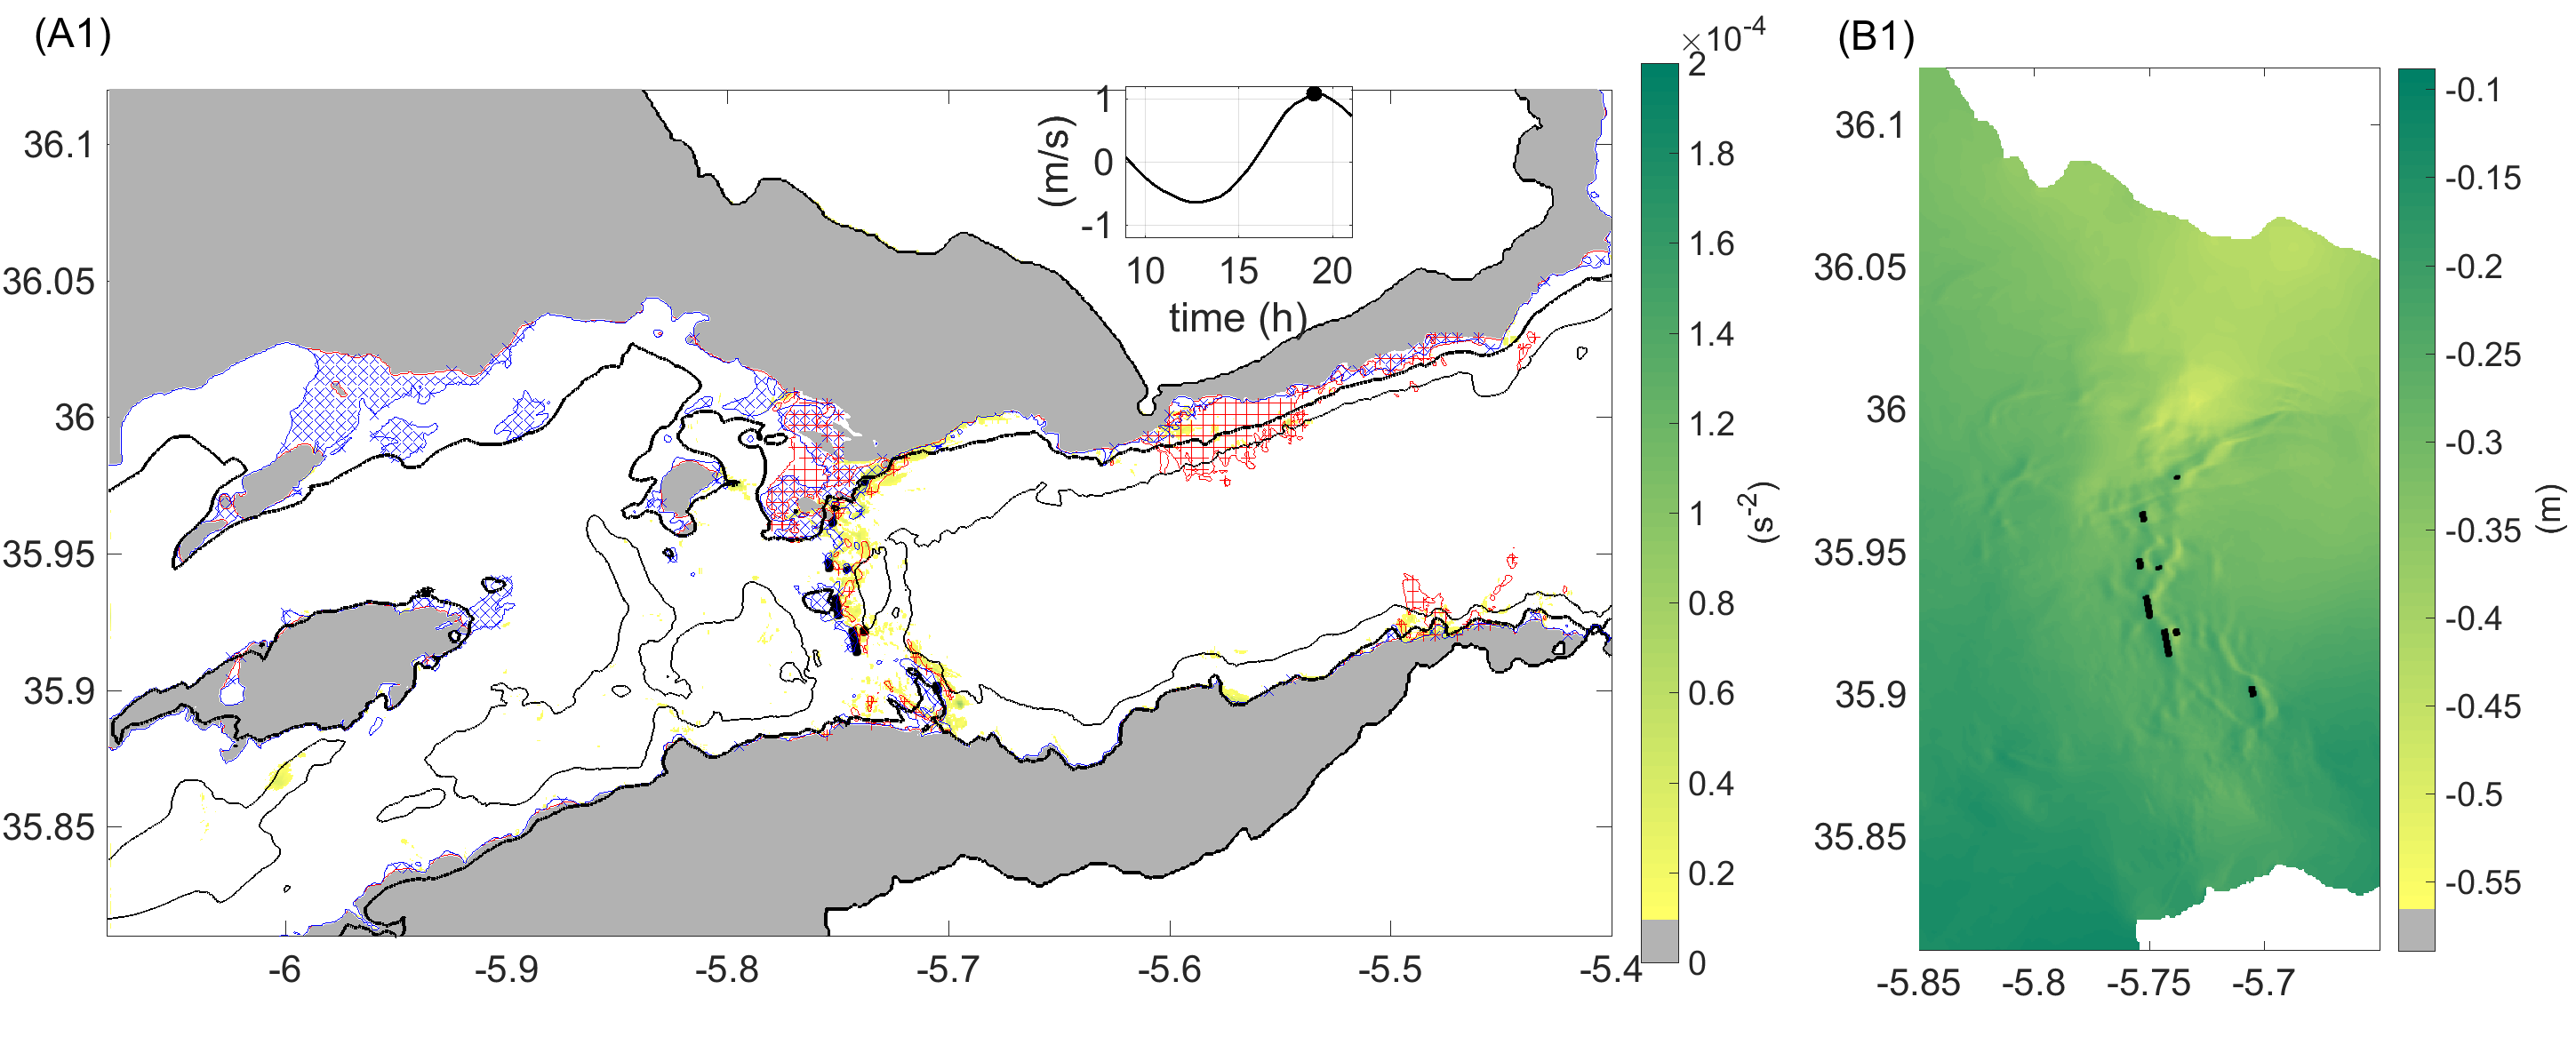
\includegraphics[width=1\linewidth]{./GBR3D/ME2_19h_p.png}
\end{subfigure}
 
 \begin{subfigure}{\linewidth}
\centering
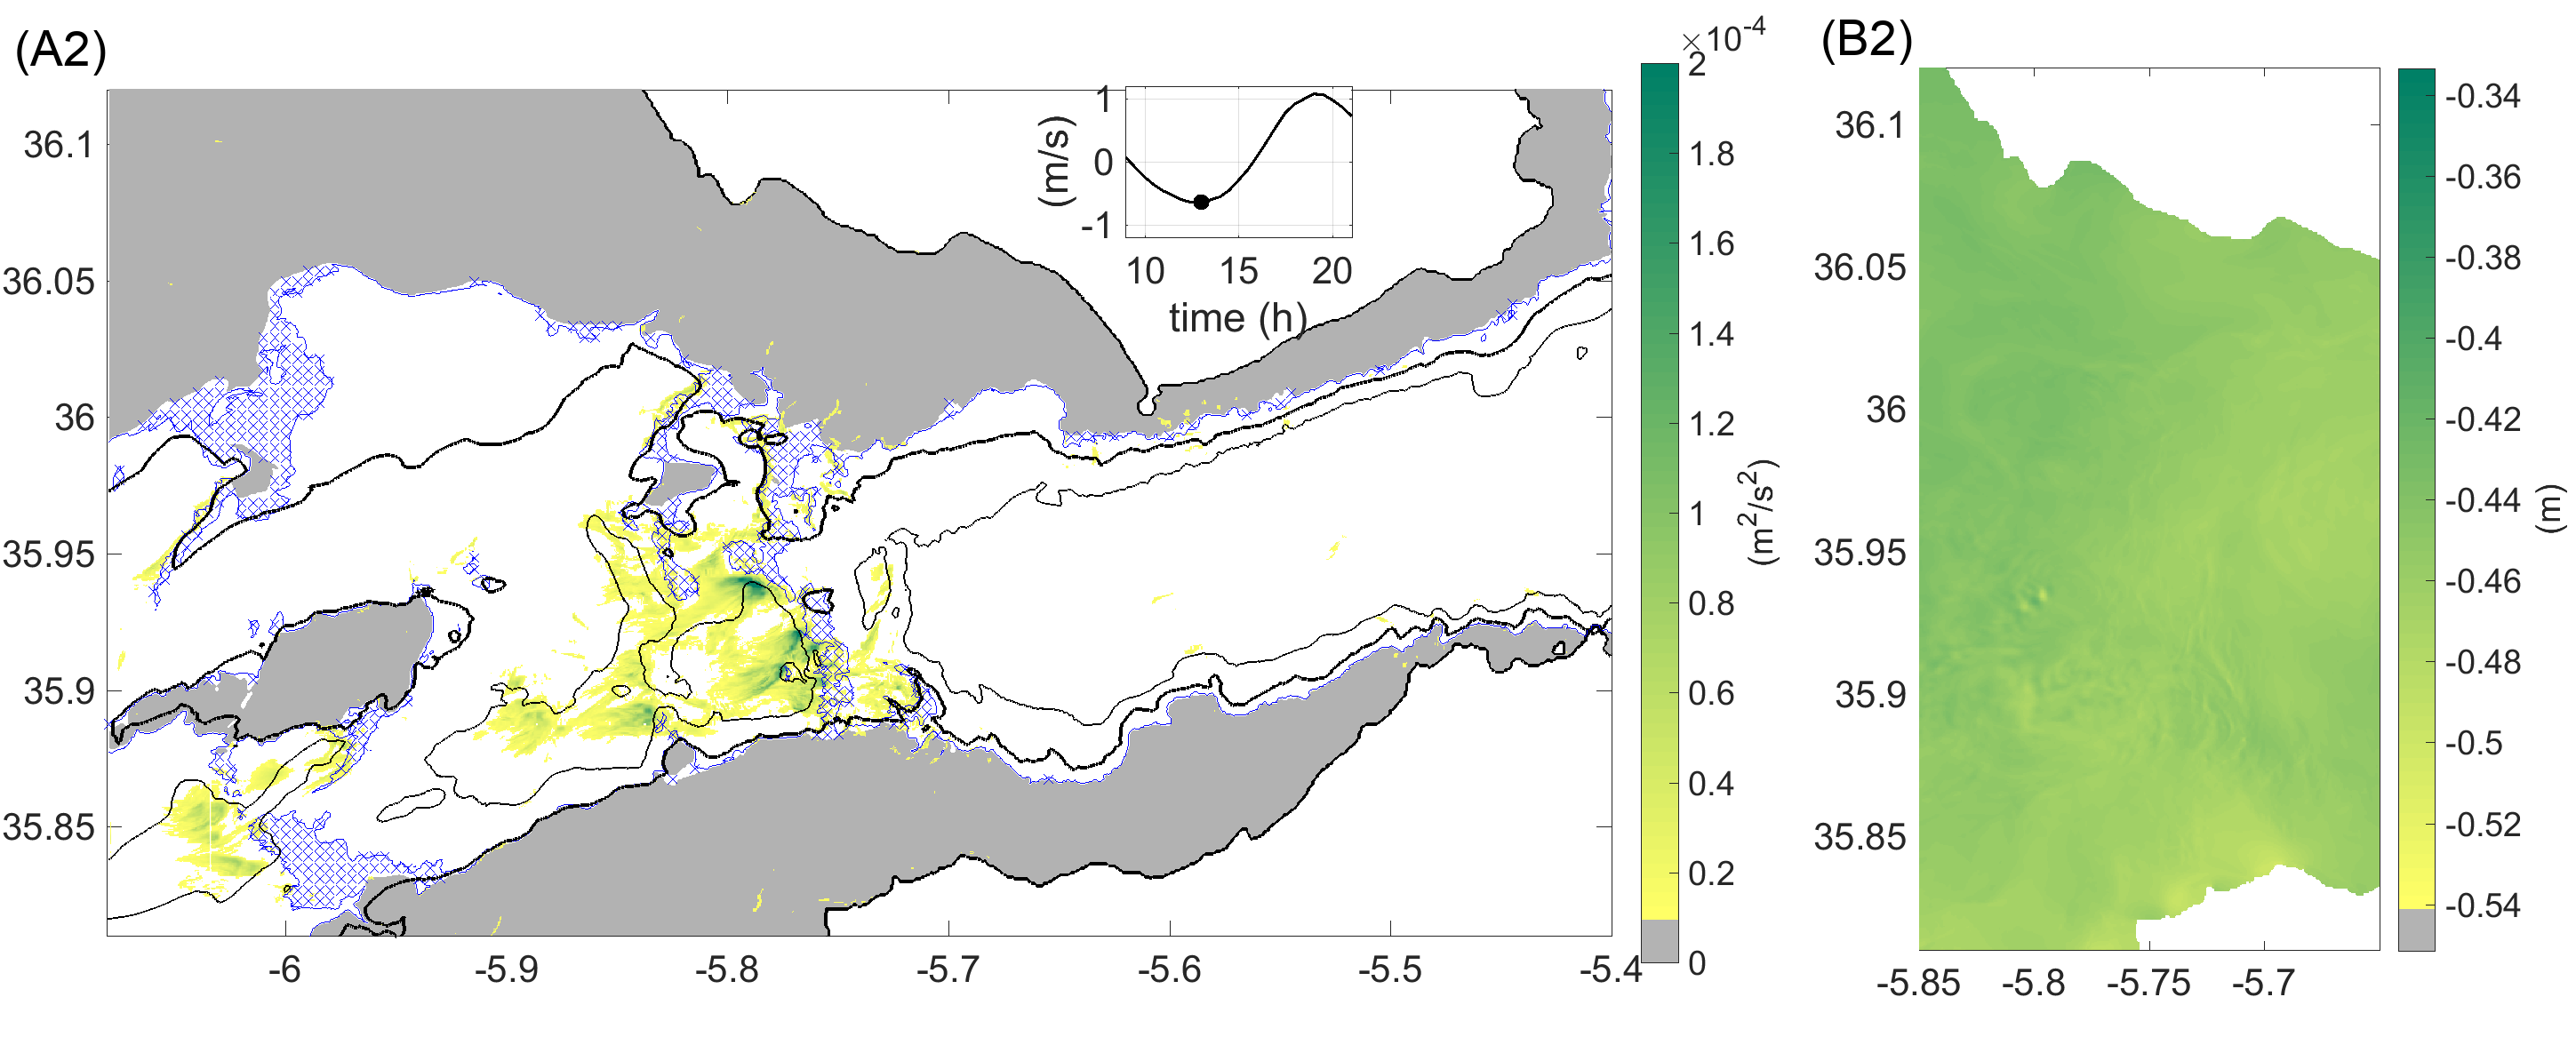
\includegraphics[width=\linewidth]{./GBR3D/ME2_13h_p.png}
\end{subfigure}
\caption {For neap tide, inflow then outflow. Blue (red) shaded area is supercritical med (atl) layer. Black dots are hyd jump detection. grey area denotes where S bottom$<$Sinterface. colorbar for . Also inicated barotropic znal current at 5.7553$^o$W  35.9238$^o$N. Two black isobathes contours are indicated, 200m (bold) and 400m(thin) depth  }
\end{figure}

\begin{figure}[!h]
 \centering
\begin{subfigure}{\linewidth}
\centering
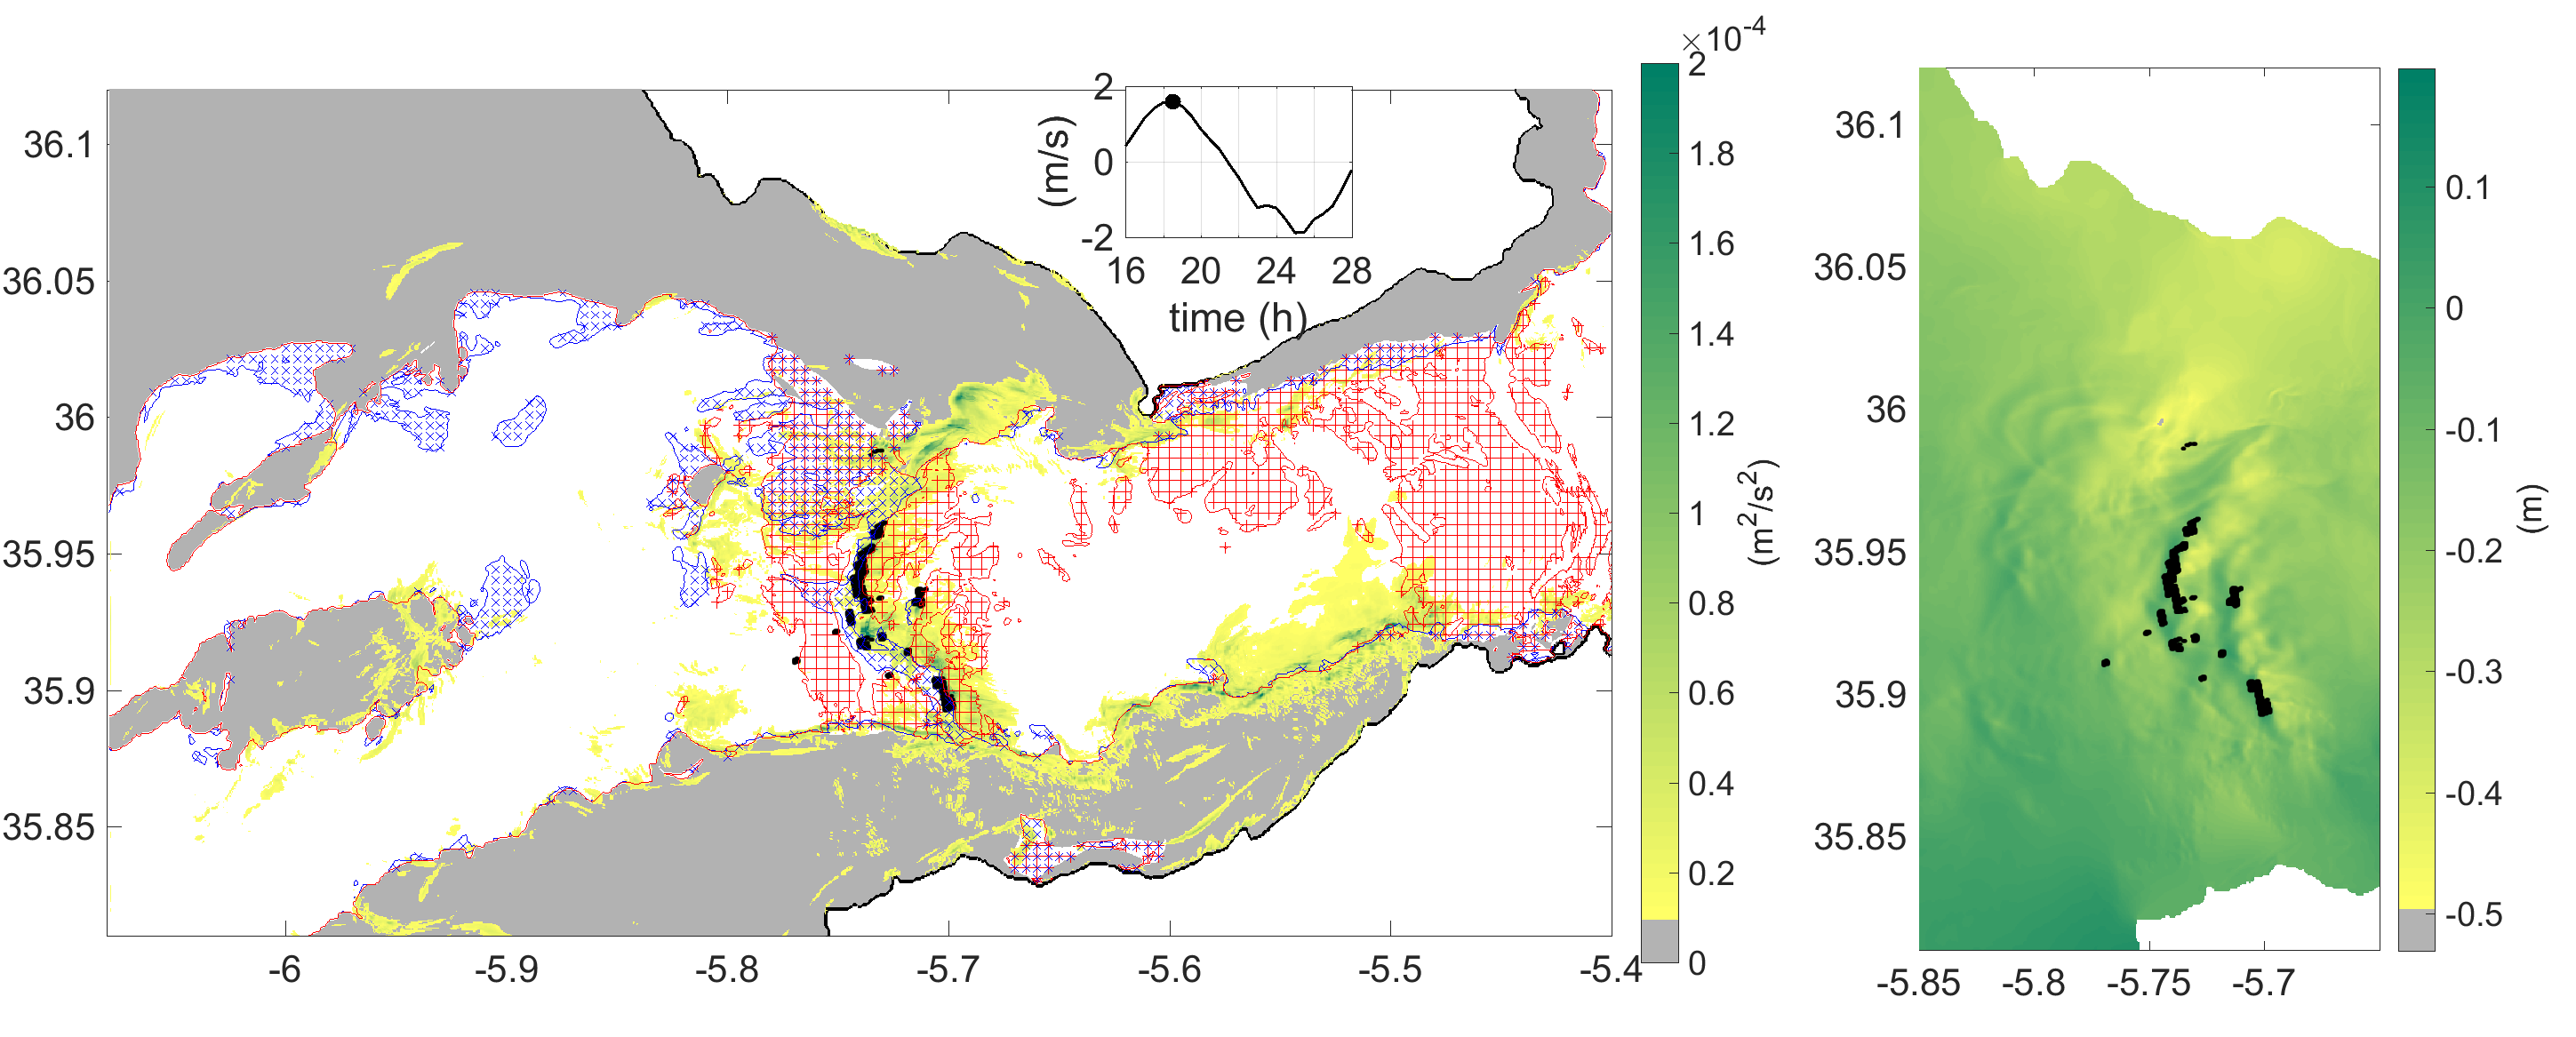
\includegraphics[width=\linewidth]{./GBR3D/VE2_18h30_p.png}
\end{subfigure}

\begin{subfigure}{\linewidth}
\centering
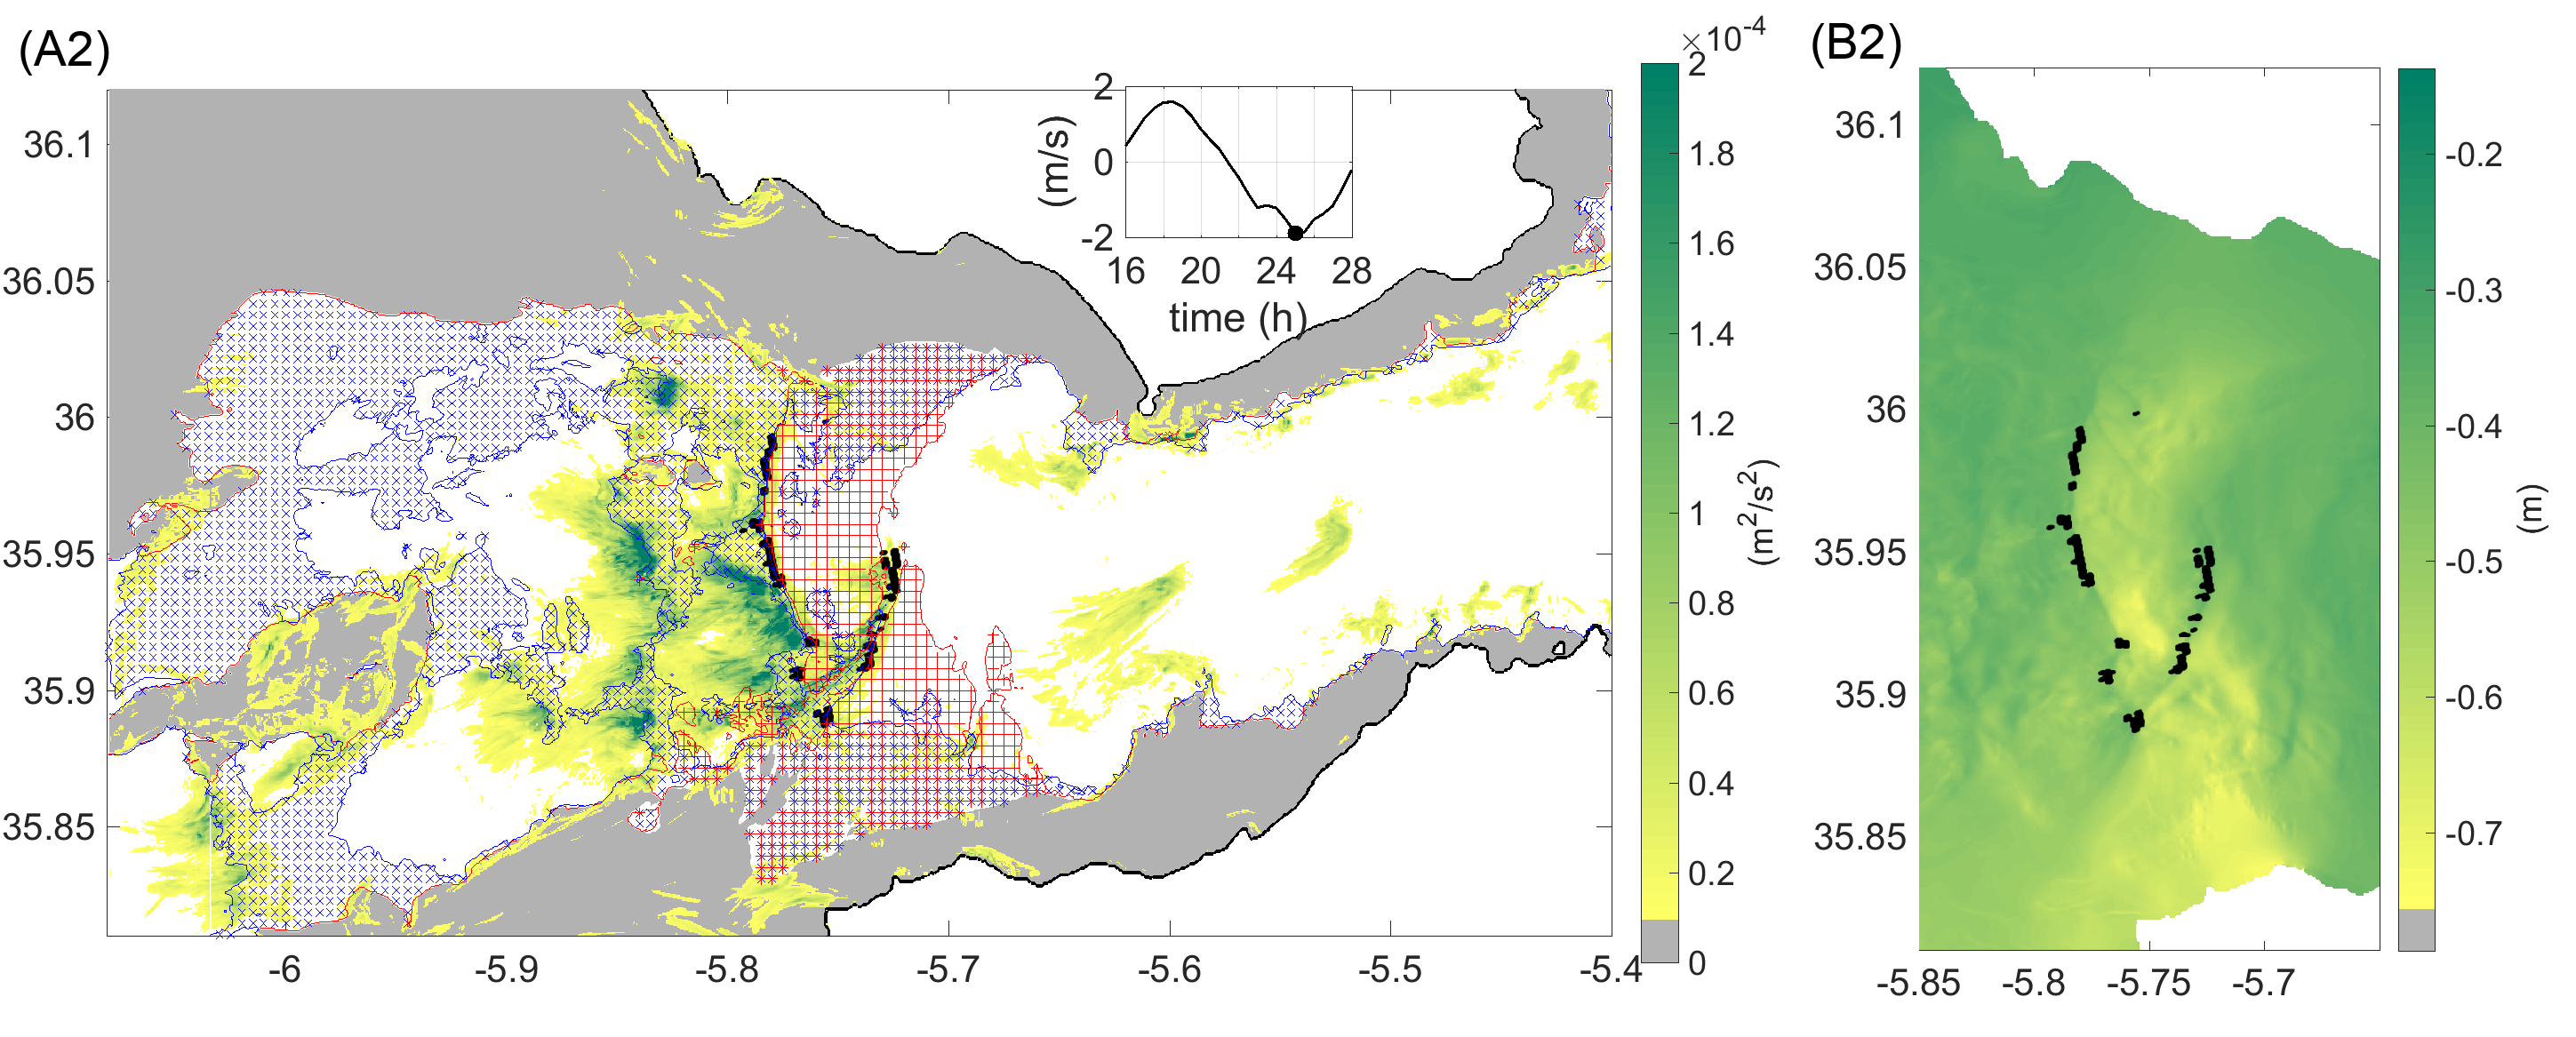
\includegraphics[width=\linewidth]{./GBR3D/VE2_25h_p.png}
\end{subfigure}
\caption {Same as figure ... for spring tide}
\end{figure}

\begin{figure}[!h]
 \centering
%\begin{subfigure}{\linewidth}
%\centering
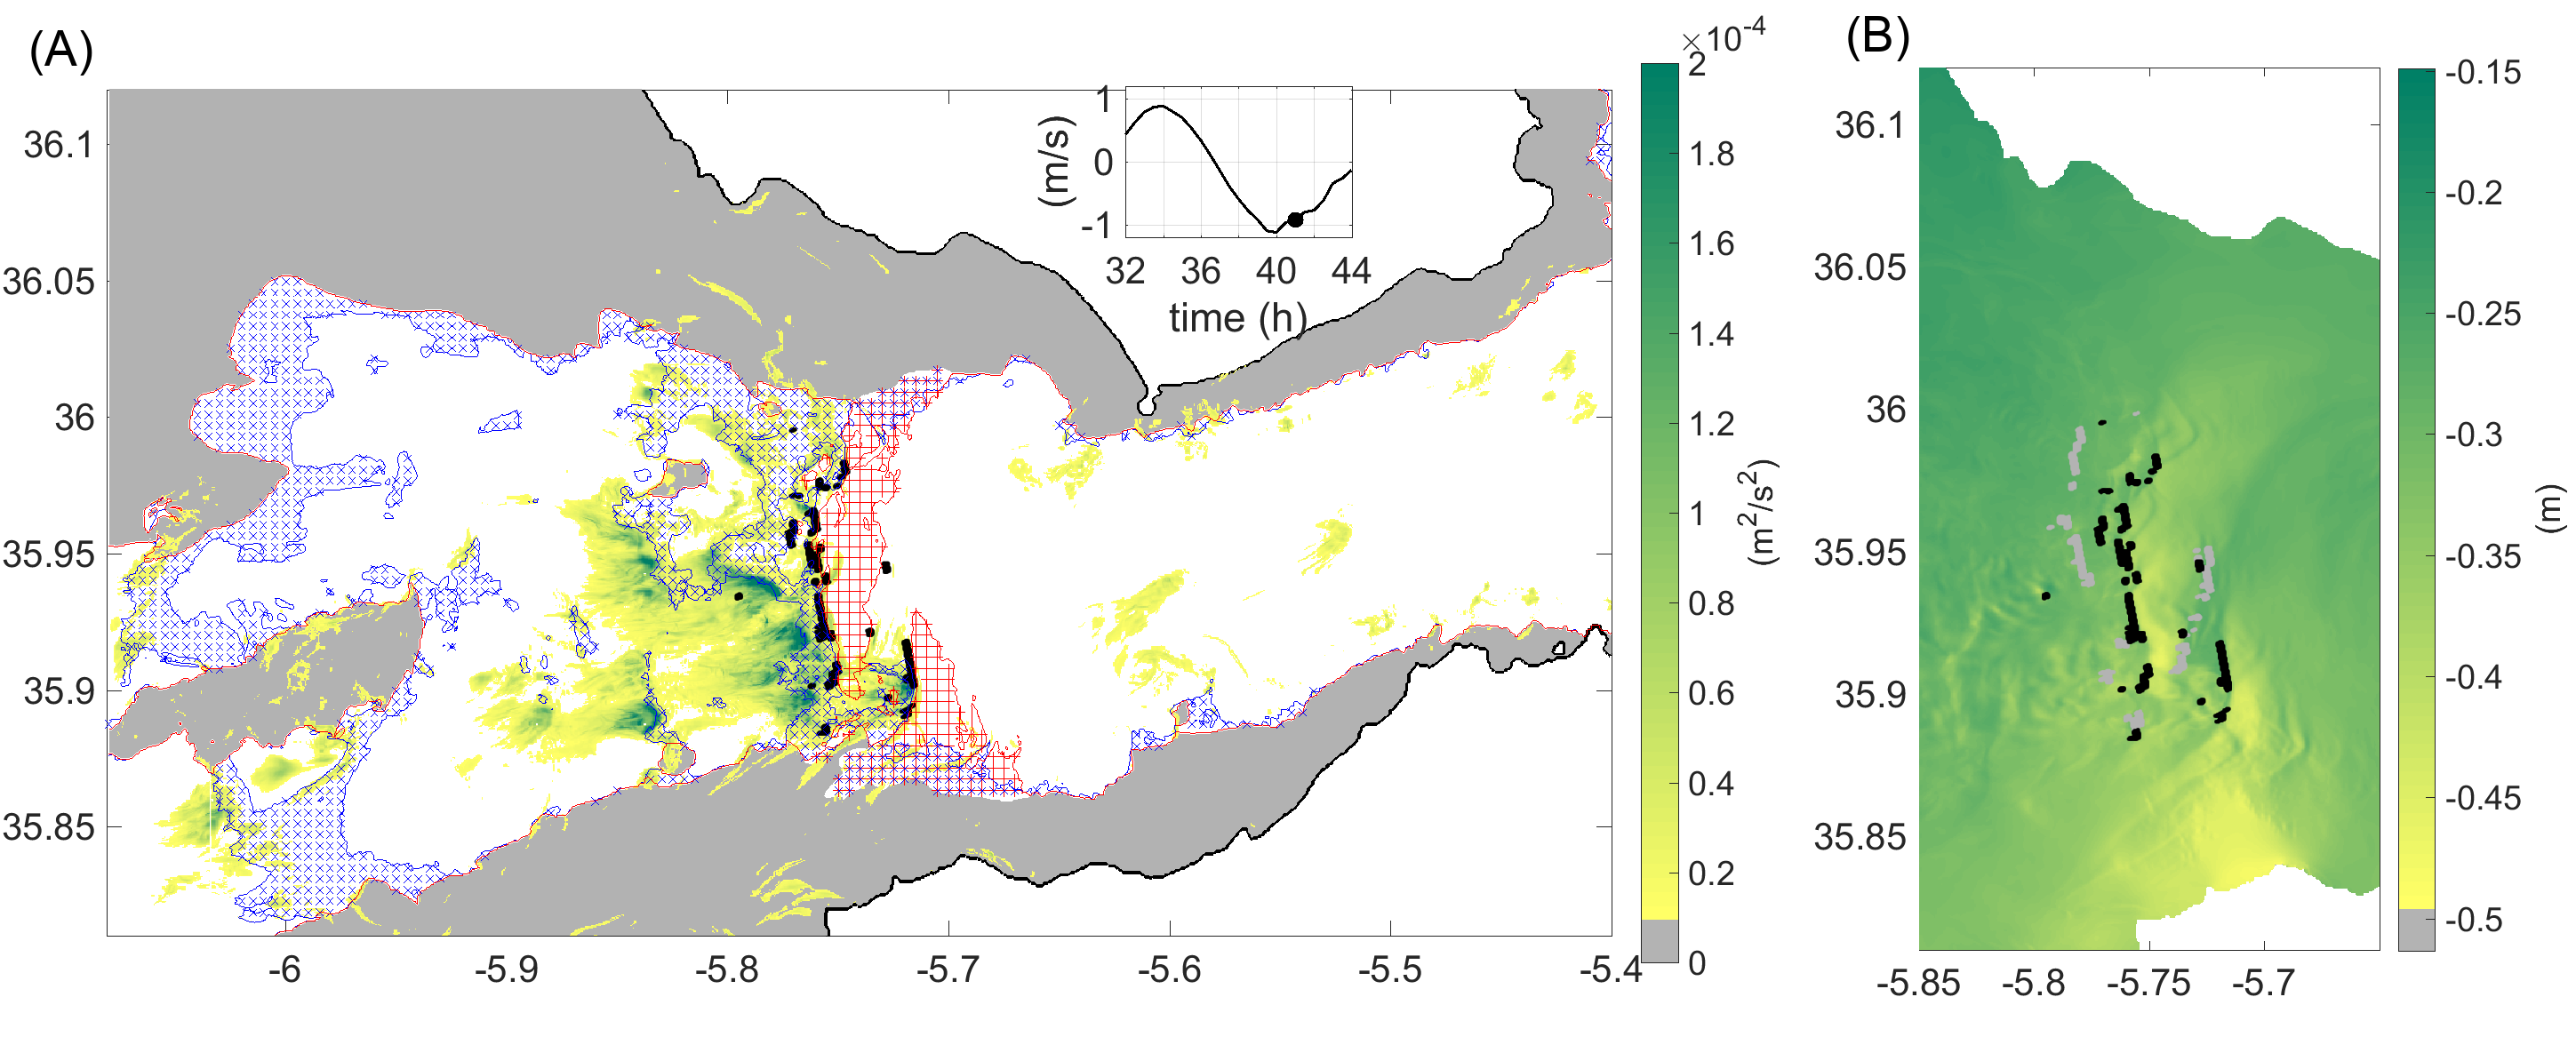
\includegraphics[width=\linewidth]{./GBR3D/IES_41h_p.png}
%\end{subfigure}
 \caption {Same as figure ... for intermediate outflow case, on figure SLA also put trace of jump of spring tide outflow}
\end{figure}




\subsubsection{Propagation of Solitons (ISWs)}

\begin{itemize}
\item Solitons dans maquette, comence avec comparaison SaR, pour comparaison choix de quel diag entre divergence  des courants, gradient de l'élévation de la surface libre
\item Simulation donne accès a plus d'information que la surface. Voudrait regarder caractéristiques des solitons qui passent en un point 
\item Présentation Matching Pursuit dans le temps, dictionnaire soliton donne amplitude, peut retrouver une vitesse de propagation
\item Comparé a ce qui a pu être observé, dans maquette toujours train ordonné...
\item donner combien d'ondes selon où dans le détroit ???
\end{itemize}


(Comp satellite, présenter MP)

Of the three period, for IT (intermediate tide), have satellite observations, SAR images . (remettre celle du poster)



Speed in the Strait, how relaxation ? Comparison velocity given by MP and propagation...


Comme son homologue à plus basse résolution NH-REF, la maquette à haute résolution NH-HR est permet de simuler la génération et la propagation des modes 1 et 2 d'ondes internes de gravité dans le détroit de Gibraltar, ce qui est en accord avec les observations des satellites Sentinel 1 et 2. De façon similaires, des ondes de grande amplitude (de l'ordre de la centaine de mètres), sont générées lors de la relaxation du ressaut hydraulique au Seuil de Camarinal. Ces ondes ont une signature de mode 1. Elles sont précédées par la propagation d'un mascaret interne puis se décomposent en train d'ondes solitaires sous l'action de la dispersion non-hydrostatique qui vient équilibrer les non-linéarités liées à l'advection. Au cours de sa propagation dans le détroit de Tarifa, ce train d'onde va en partie se réfléchir sur les côtes en train ondes se propageant vers l'ouest. Afin de détailler l'apport de l'augmentation de la résolution sur ces ondes, la figure \ref{fig_mod1_HR-REF}.a présente une coupe verticale en densité du train d'ondes solitaires alors qu'il entre en Mer d'Alboran dans la maquette NH-HR (en couleur) et dans la maquette NH-REF (en pointillés). \\
Les ondes de mode 1 se sont propagées plus vite dans la maquette NH-HR, et le nombre d'ondes dans le train est plus grand (5 contre 2). Ce comportement est le même à chaque période de marée et la variation du nombre de solitons d'une période de marée à une autre peut être simulée avec la maquette NH-HR. Cette forte variabilité diurne est illustrée dans le tableau \ref{tab_XEC}, réalisé en notant l'arrivée de l'onde de mode 1 au point le plus à l'est dans la figure \ref{fig_mod1_HR-REF}.a (ou à tous les points de la figure \ref{fig_mod1_HR-REF}.b pour le calcul de la vitesse de propagation). Les vitesses les plus fortes dans ce tableau correspondent à une advection par des courants de marée plus importants, on observe que ces périodes sont associées à un plus petit nombre d'ondes dans le train avec une périodicité elle aussi plus petite. Il est à noter que ces valeurs ne sont pas identiques pour toutes les latitudes à la sortie du détroit: du fait de la dispersion induite par la force de Coriolis, l'amplitude de la première onde est par exemple plus grande dans la partie sud.








\subsubsection{Génération de tourbillons dans le sillage des solitons}

\begin{itemize}
\item Voit tourbillon dans la maquette... effet sur le train de soliton
\end{itemize}


Les simulations NH-REF et NH-HR montrent la génération d'un tourbillon au passage des trains de solitons à la sortie du détroit. Cette génération pourrait être une conséquence des violents cisaillements de courants horizontaux générés par l'onde interne.\\
La structure tourbillonnaire demeure dans cette région puis déforme le train d'ondes solitaires suivant. A notre connaissance, il n'existe pas d'observations ni de preuves directes de son existence.\\
Son impact sur les solitons n'est toutefois pas négligeable puisque les simulations numériques montrent pour certaines périodes de marées une désorganisation du train d'ondes solitaires à la sortie du détroit. Cette déstructuration du train d'ondes solitaires pourrait être une conséquence de son interaction avec le tourbillon suivant ou être associée à la génération de la structure tourbillonnaire. Ces conséquences ont été observées par (Vlasenko et al., 2009) et pourraient quoiqu'il en soit confirmer indirectement la présence de la structure tourbillonnaire. Il convient toutefois d'être prudent et de nouvelles investigations sont actuellement en cours afin de préciser le mécanisme de génération du tourbillon et de rassembler des observations in situ pouvant confirmer sa présence.





\subsubsection{Dynamic at Camarinal Sill, simu VHR 50m}

\begin{itemize}
	\item Exemple domaine Cso et diagrammes TS entre zones où insta se developpent (diag TS, std, trace svd et histogrammes, montrer les vecteurs temps des premieres EOF et EOF de cell où insta en 3D)
	\item Variabilité marée, voit difference emplacement selon maree (pas diag T,S dispo mais pas les même situations donc comparaisons bof.)
	\item Effet simu num, schéma de fermeture etc, sur premier outflow IES (voit effet salinité, dynamique différente des instabilités)
	\item Selon comment simule le passage, caractéristique de la veine med différentes...
\end{itemize}


Camarinal Sill, concerning the Mediterranean outflow, it is the first pace where it is 'formed' (for atl waters, already processes before it reaches CS that will mix it...). Further along on the med outflow pathways, the characteristics of med outflow result from accumulated changes , so more difficult interpretation.  As seen previously, at CS, instbailities. Furthermore, flow has variability. Here we showcase variability of the neap-spring tide cycle. Another point is the turbulence closure scheme.

Use simulations with S 0.005 then S var or K-ep

(que simus 50m)



How the shape of the hyd control influences the passage, compare east and west of the sill... 
Those waters flowing west of the sill are result of mixing with Atl waters at the sill's passage.
In certain case, water flowing westward is saltier and colder, which may be interpreted as a greater part of original med water masses in the mix.


Explore how the passage of the sill takes place in simulations.



\subsubsection{Primary shear instabilities  (non general paragraphe avant, met cette partie avec reste la parle ressauts etc...}

Mettre coupe avec/sans ressaut, comp les 3 cas...

\begin{itemize}
\item Cisaillement passage de seuils car accélération veine med et accélération supplémentaire avec couranst de marée : cascade turbulente avec développement instabilités de cisaillement (ou point expliqué dans partie antérieure/biblio???)
\item Le début de ces isntabilités/instabilités primaires/début de la cascade est simulé dans modèle non hydrostatique. Orécédemment a été montré dans simus 2D, ici 3D
\item Pour repérer ces instabilités, utilise le calcul de l'invariant Q (exemple de coupe où on voit aussi le 'rouleau' d'eau interfaciale et contour Q$>$Qa). Voit les rouleaux êtres advectés
\item 2 statistiques effectuées : on line (sur 30 minutes), calcul de la standard deviation / ecart type max dans la colonne d'eau de Q. Comme a advection des instabilités primaires, en un point voit oscillations haute fréquence
\item SVD comme pour chap 2D. Sauf que traitement off line nécessite d'avoir sorties 3D hautes fréquences, vite des fichiers lourds
\item Montre exemple d'un EOF (montre celui qui a de la HF, EOF précédents liés mouvement du ressaut), mêmes emplacements ou a ecart type grand. Ici EOF que sur partie Camarinal, montre carte ecart type voit aussi ES et a trace du déplacement du soliton.
\item Partie suivante voir plus sur CS, la variabilité.
\item PEut ajouter un mot sur le fait que voit effet mélange dans diagramme T,S
\end{itemize}

La sortie des eaux Méditerranéennes au détroit de Gibraltar commence par le passage du Seuil de Camarinal. A cet endroit, la veine Méditerranéenne est accélérée sous l'effet de la topographie et des courants de la marée barotrope semi-diurnes. Cette accélération peut amener à la formation d'un ressaut hydraulique à l'aval duquel les eaux méditerranéennes sont mélangées. 

The (primary) instabilities in the jump at CS were numerically represented in a 2D non-hydrostatic high resolution model of the Strait ( Hilt et al 2020), they will also be explicitely represented in a realistic 3D model, and can look at their repartition/general behaviour. Just as used Okubo-Weiss in Hilt2020, naother tracer of the rotation of the instabilities can be used : the Q-parameter (Kolar2011).

Figure ... is an exemple of the value of $Q$ in 3D simulation where localisation of $Q>Q_a$ is compared at t=$x$h to $u$ (ou u moins u barotrope?) and salinity $S$. Can see area of minimum $S$, when look at next iterations of the simulation, see this 'rolls' are being advected by the med flow westward. 


\begin{figure}[!h]
 \centering
 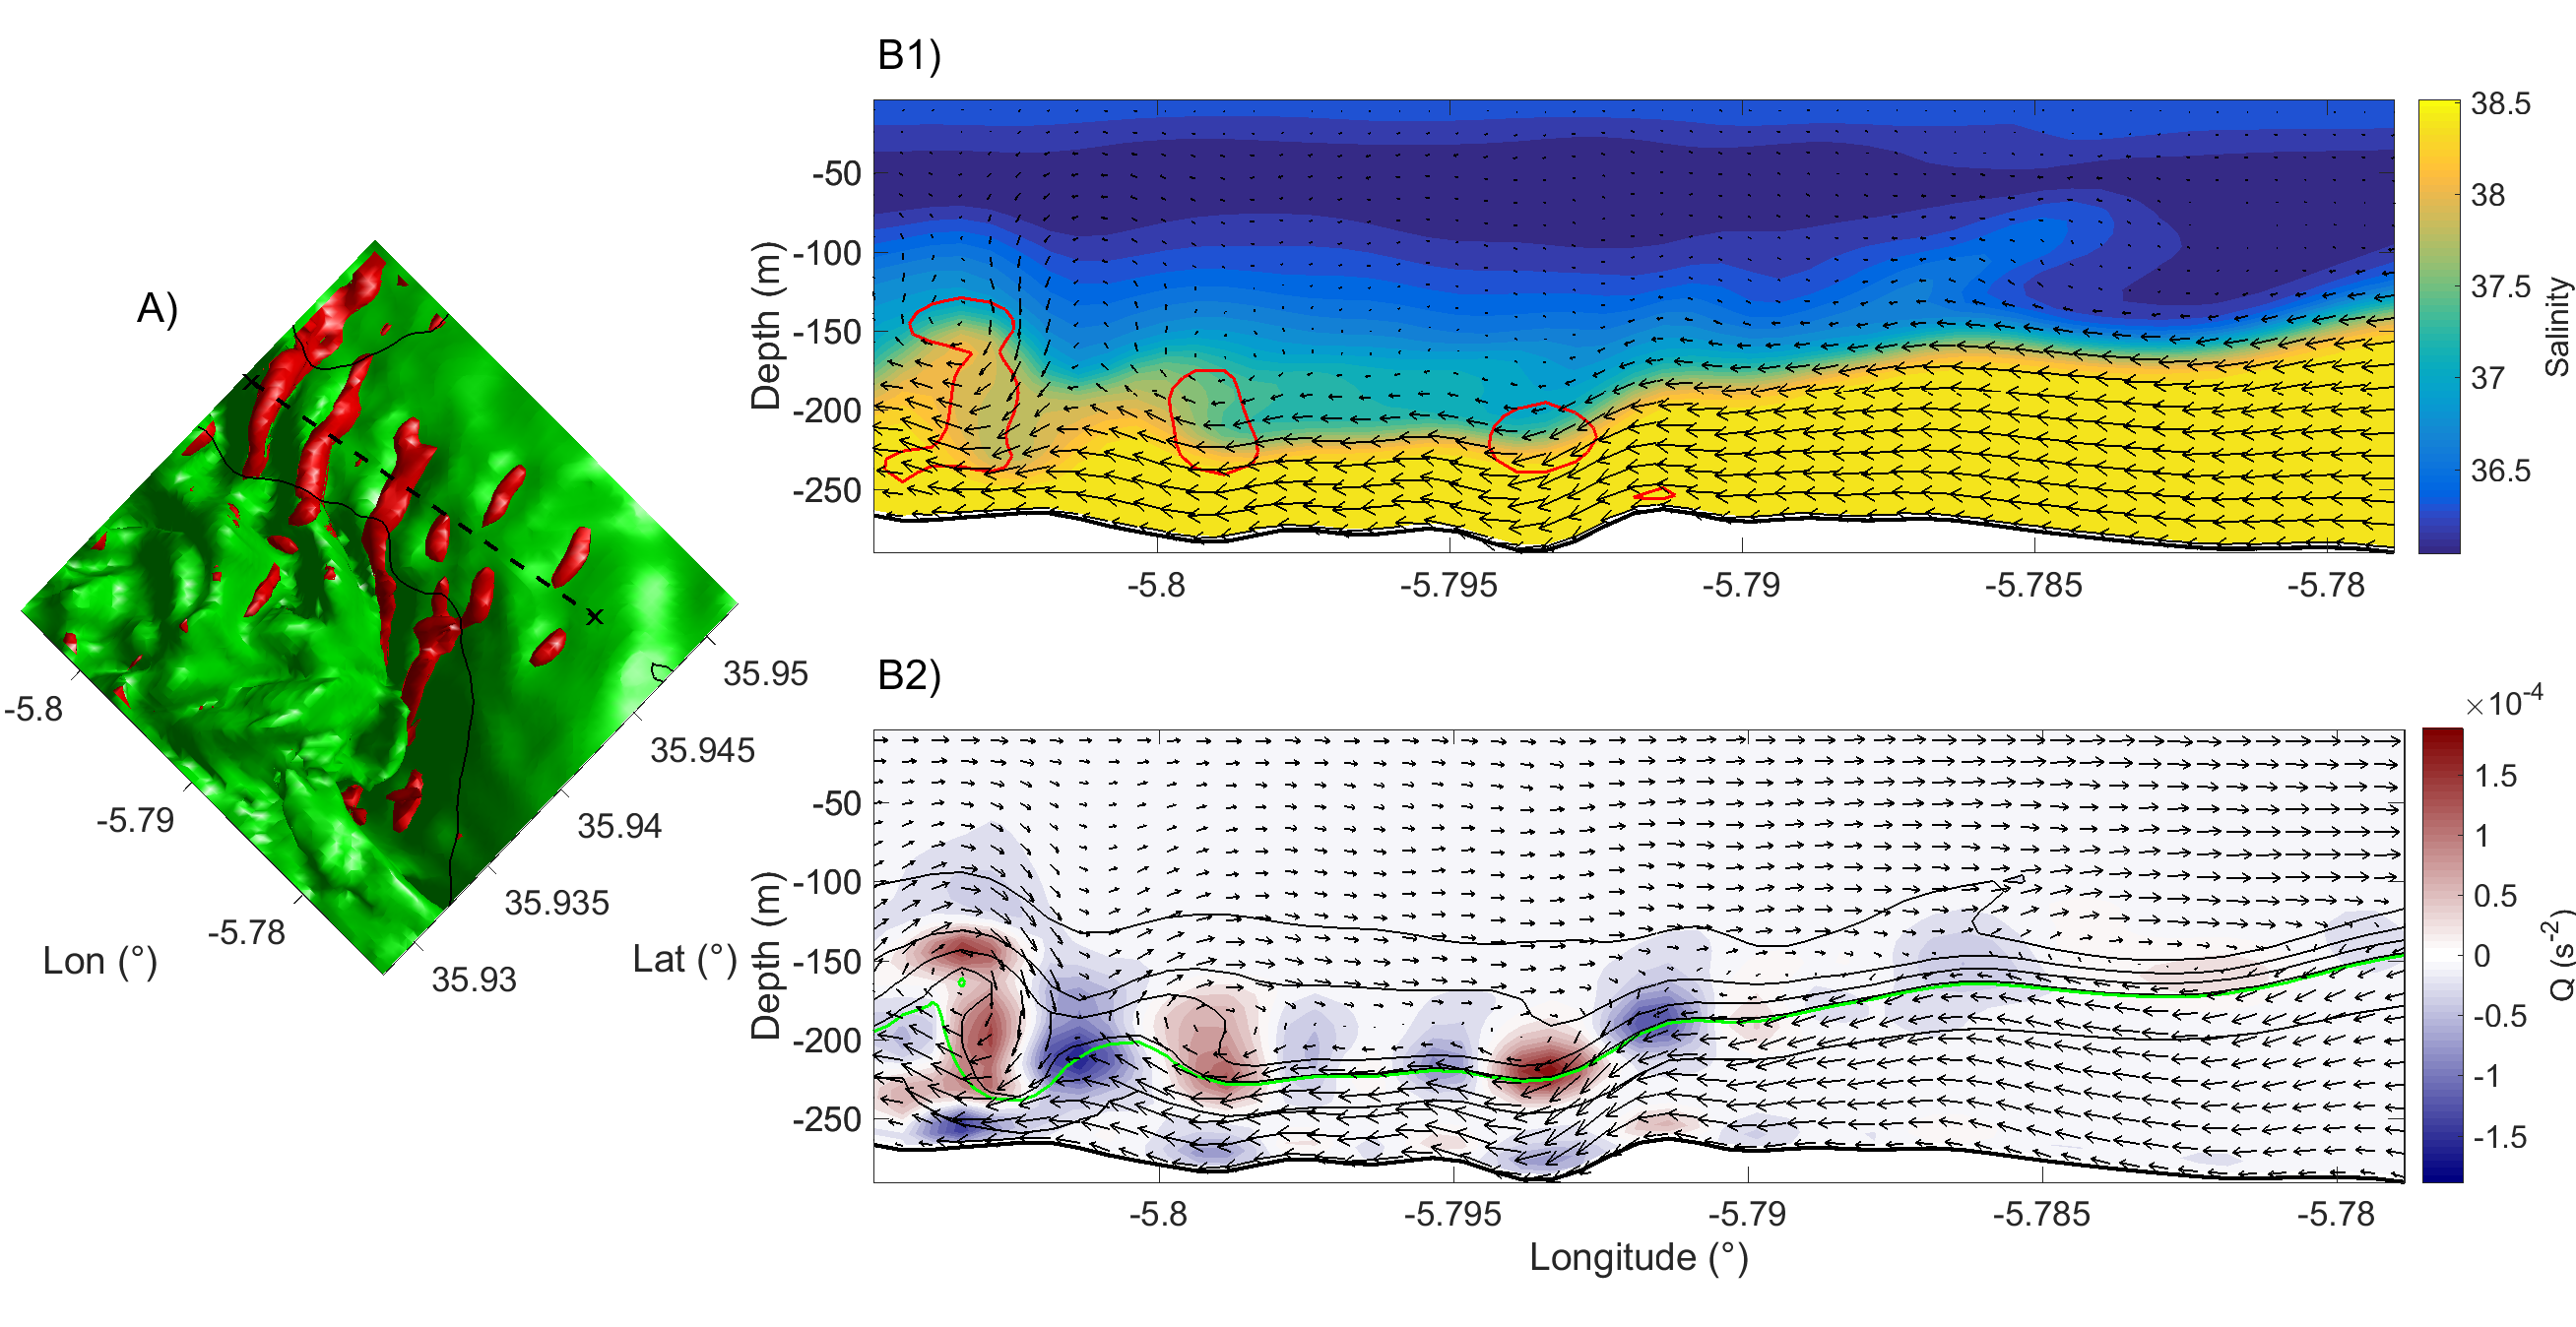
\includegraphics[width=1\textwidth]{./GBR3D/FigInstaQ_IES4H.png}
 \caption {(a) Vue zénitale d'isosurfaces de salinité $S=38.1$ (verte) et d'invariant $Q=5.10^{-5}$ (rouge) dans une zone à l'ouest du Seuil de Camarinal, Détroit de Gibraltar. Isobathe 300 m (trait plein) et trace de la section des coupes verticales (b) et (c) (trait pointillé). (b) Section veticale de salinité (couleur), vecteur des composantes (u,w) du courant et isocontours de l'invariant $Q=5.10^{-5}$ (rouge). (c) Szection verticale de l'invariant Q (couleurs), isohalines (trait noir et trait vert $S=38.1$), et vecteurs des composantes (u',w) où u' est le courant dans la direction longitudinale moins sa composante barotrope.}
 \label{figdraftQ}
\end{figure}





In (next part), look at the influence of tidal cycle (and so of hydrauli jump) and numerical choices, on the instabilities at area of Camarinal Sill.

(diag T,S a longitude constante selon region avant/apres les instabilites....)





%-------------------------------------------------------------------------------------
%\subsection{Results}

%Section discussion physique du detroit dans les maquettes 50m

\subsubsection{Water mass mixing near/downflow of Camarinal Sill}

Take a result in spring tide case (S0.05), figure std(Q) of last part zoom in on Camarinal Sill area. Green inset is area where SVD is performed, can see hotspots of high std correspond with trace of the spatial EOF field of Q. Trace T,S diagrams in between areas where those instabilities develop. See the transformations happen mostly between areas where instabilities, otherwise signal eroded as outflow makes its way by entrainment and circulation in shallower parts of the strait that leave the coldest, saltiest waters behind.

\begin{figure}[!h]
% \centering
 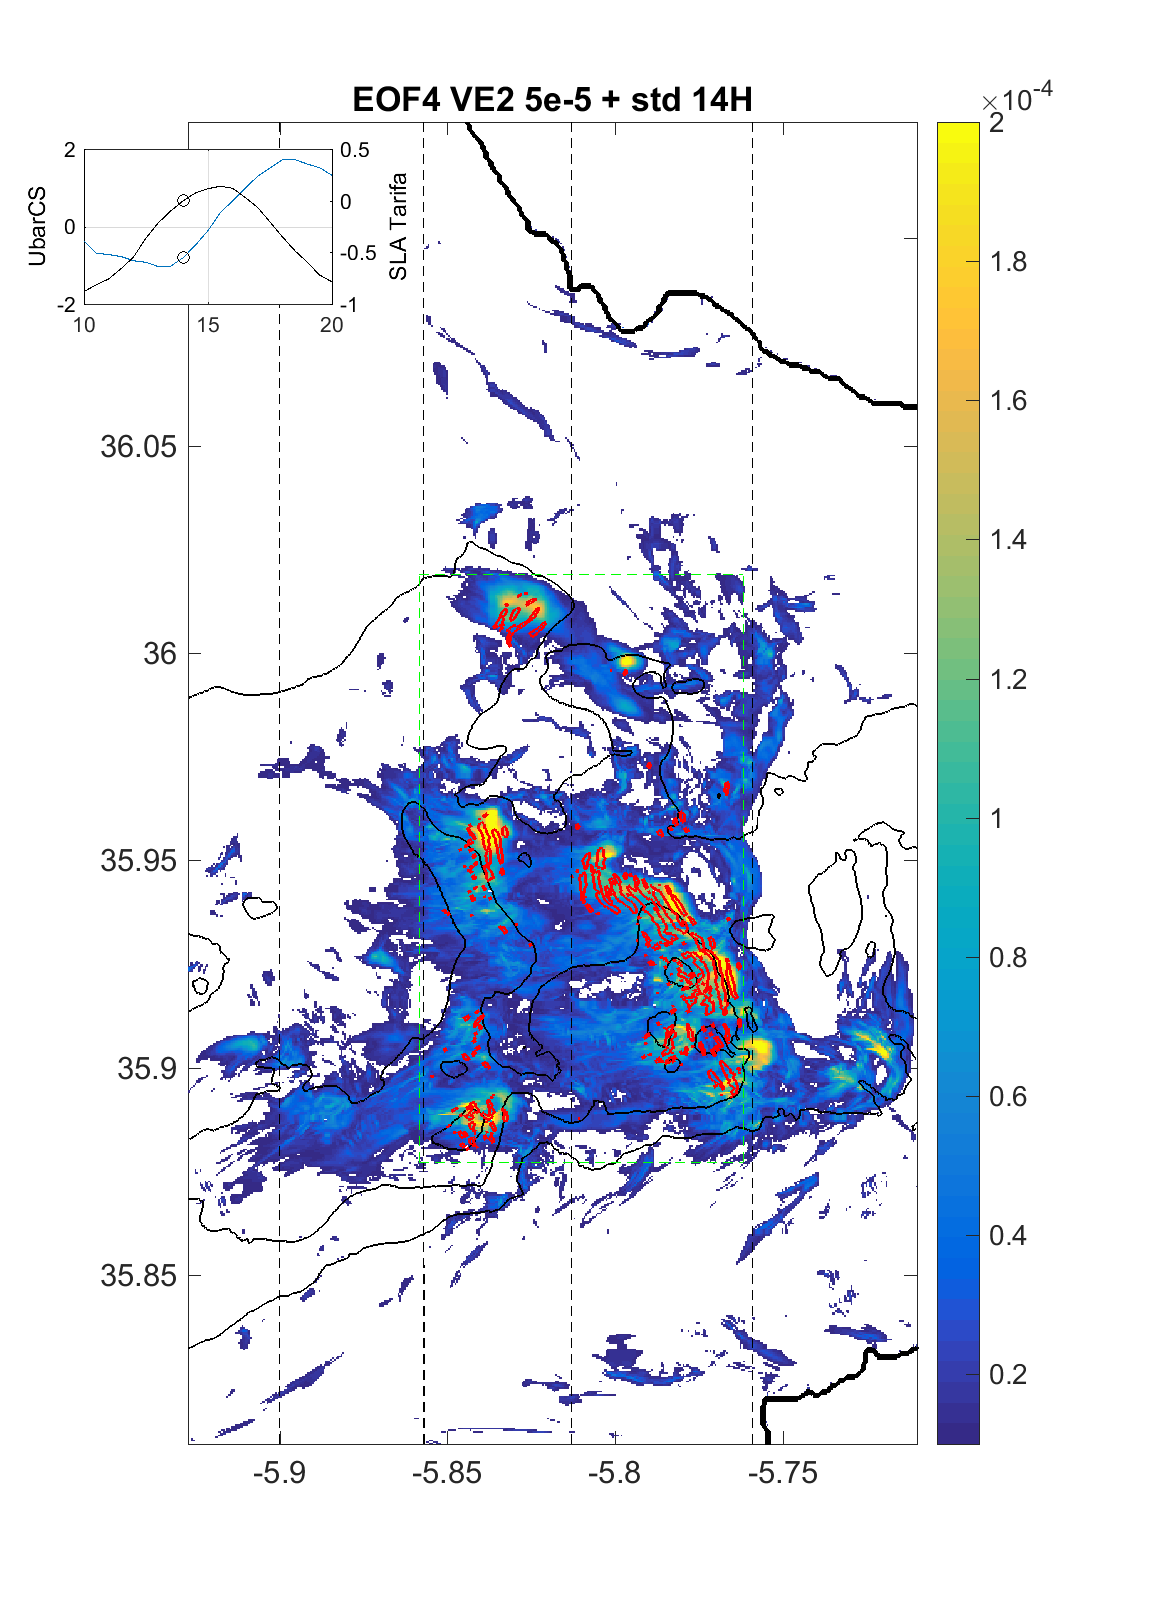
\includegraphics[width=0.3\textwidth]{./GBR3D/EOF_std_14hCso_traces.png}
 \caption {std(Q) in last 30 minutes before 14H of simulation time in spring tide simulation, and trace of contour Q of SVD}
\end{figure}

\begin{figure}[!h]
% \centering
 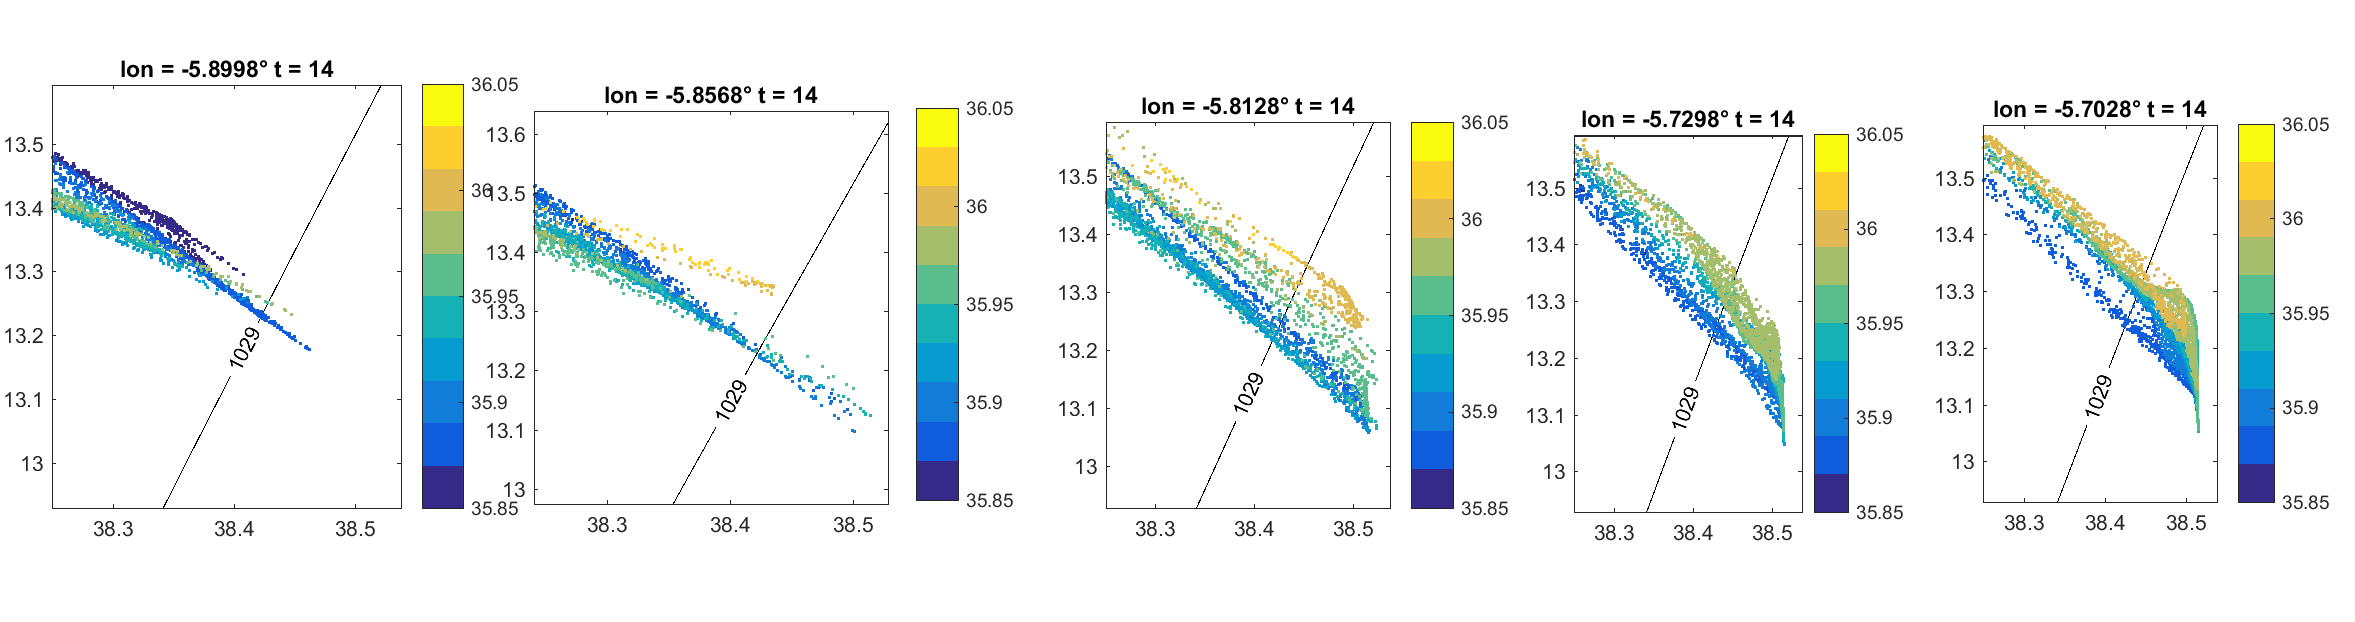
\includegraphics[width=\textwidth]{./GBR3D/TS_coupesCso14h.png}
 \caption {T,S diagrams, inset on med outflow area}
\end{figure}

Look at the area where the first instabilities are developped in med outflow.

\subsubsection{Neap-spring tide variability}
\subsubsection{Mediteranean pathways and hydraulic jump at Camarinal Sill variability(dans partie precedente?)}

Flow in the Strait is constrained by hydraulic controls at several points. The major one is Camarinal Sill.

The outflow of Med waters at CS is intermitent
West a reservoir , in outflow period add Med waters.




\subsubsection{Primary instabilities variability}

(S0.05), look at the three different outflow case of part ... and do SVD of Q parameter on area of the CS and directly downflow. (rajoute trace std???) Select the first EOF for which signal in the right hand side vector (that defines temporal evolution of the EOF) is high frequency, in each case the fifth, for the four others more lower frequency associated with the general flow, except for neap tide outflow that retains/superposes high frequency. Figure ... presents the left-hand side (spatial structure) term as the zenithal contour for tha value Q ... , as well as histogram of points that have value gerater than Qp. For each case center of the Q vortexes are 100m above seafloor, a bit less in neap tide case reflecting the height of the mediteranean outflow.


\begin{figure}[!h]
% \centering
 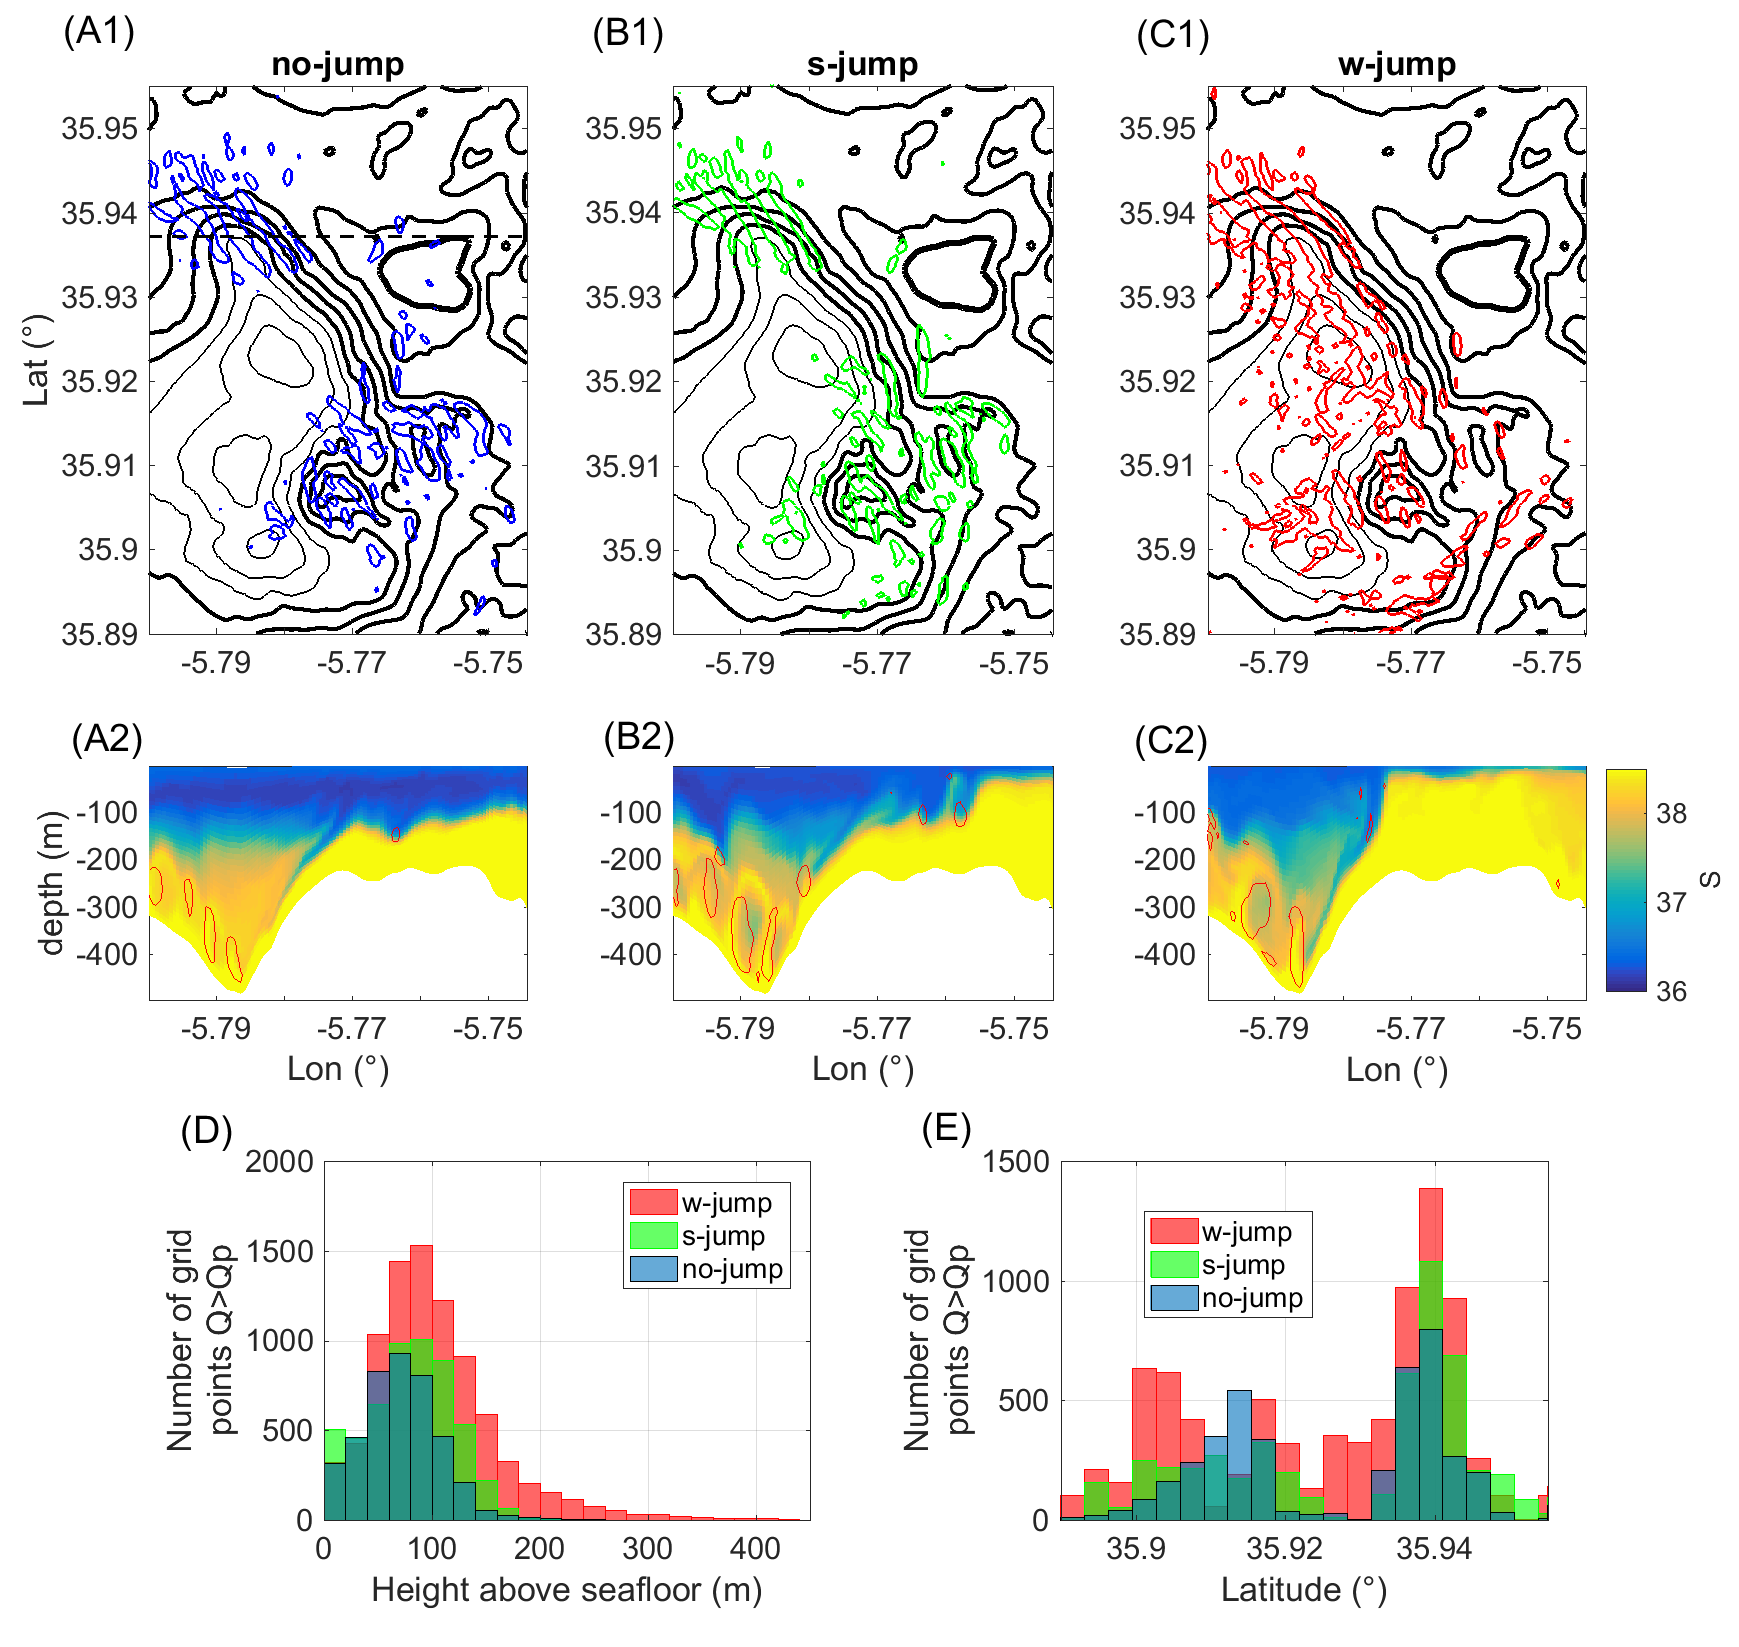
\includegraphics[width=\textwidth]{./GBR3D/EOF5_MIV_2D.png}
 \caption {}
\end{figure}

(mettre effet sur mélange diag T,S ici plutot.... a CSo aussi long ? ou s'en fout...


\subsection{Closure scheme}

\begin{itemize}
\item Situation de la comparaison : Simu IES, premier outflow, ressaut a l'aplomb seuil (?)
\item Comparaison, Smago avec coefficient horcon 0.001 ou 0.01 ou 0.1  et GLS Kepsilon
\item coef Smago plus grand, prend moins d'eaux de la pycno injectée dns la veine, med outflow plus salé, Kepsilon enter cas 0.001 et 0.01, discuter pourquoi ce sdifférences
\end{itemize}

The behaviour of the hydraulic jump changes with the parametrisation chosen... Case S0.001 instabilities devlop from the inset of the jump at approx 5.77 deg and the billows contain less salty waters, ie the signal of atl surface water in the med outflow will be stronger in this simulation.


While the width of the Med vein as it begins to go downslope of Camarinal as salty water is the same, in simulations 1 and 2 instabilities are earlier in the jump and bring more atl waters as the core or billows are advected downslope, resulting in more atl water being integrated to the med outflow at the passage of CS. Figure gives the average salinity of the med outflow taken at lon ... averaged over all latitude (med outflow defined by all parcels of salinity superior to interface smlinity...).

Looking at condiftions for the instability development, richardosn number (computed on 1h averaged field to filter the billows) is below 0.25 for each simulation, however, looking more in detail the shear and stratification, stratification is more or less teh same but shear is lesser in 3.

This is counterintuitive as 3 has a greater diffusivity and viscosity, this acts without instabilitied for exemple like east of the sill in figure with enhancing mixing in the haloclyne with surafce waters becoming saltier and deep waters becoming less salty.

Kepsilon on the other hand see less developped roll of salinity although the instabilities begin at ... On average this seems to lead to a slightly less salty mediterranean vein.


\begin{figure}[!h]
% \centering
 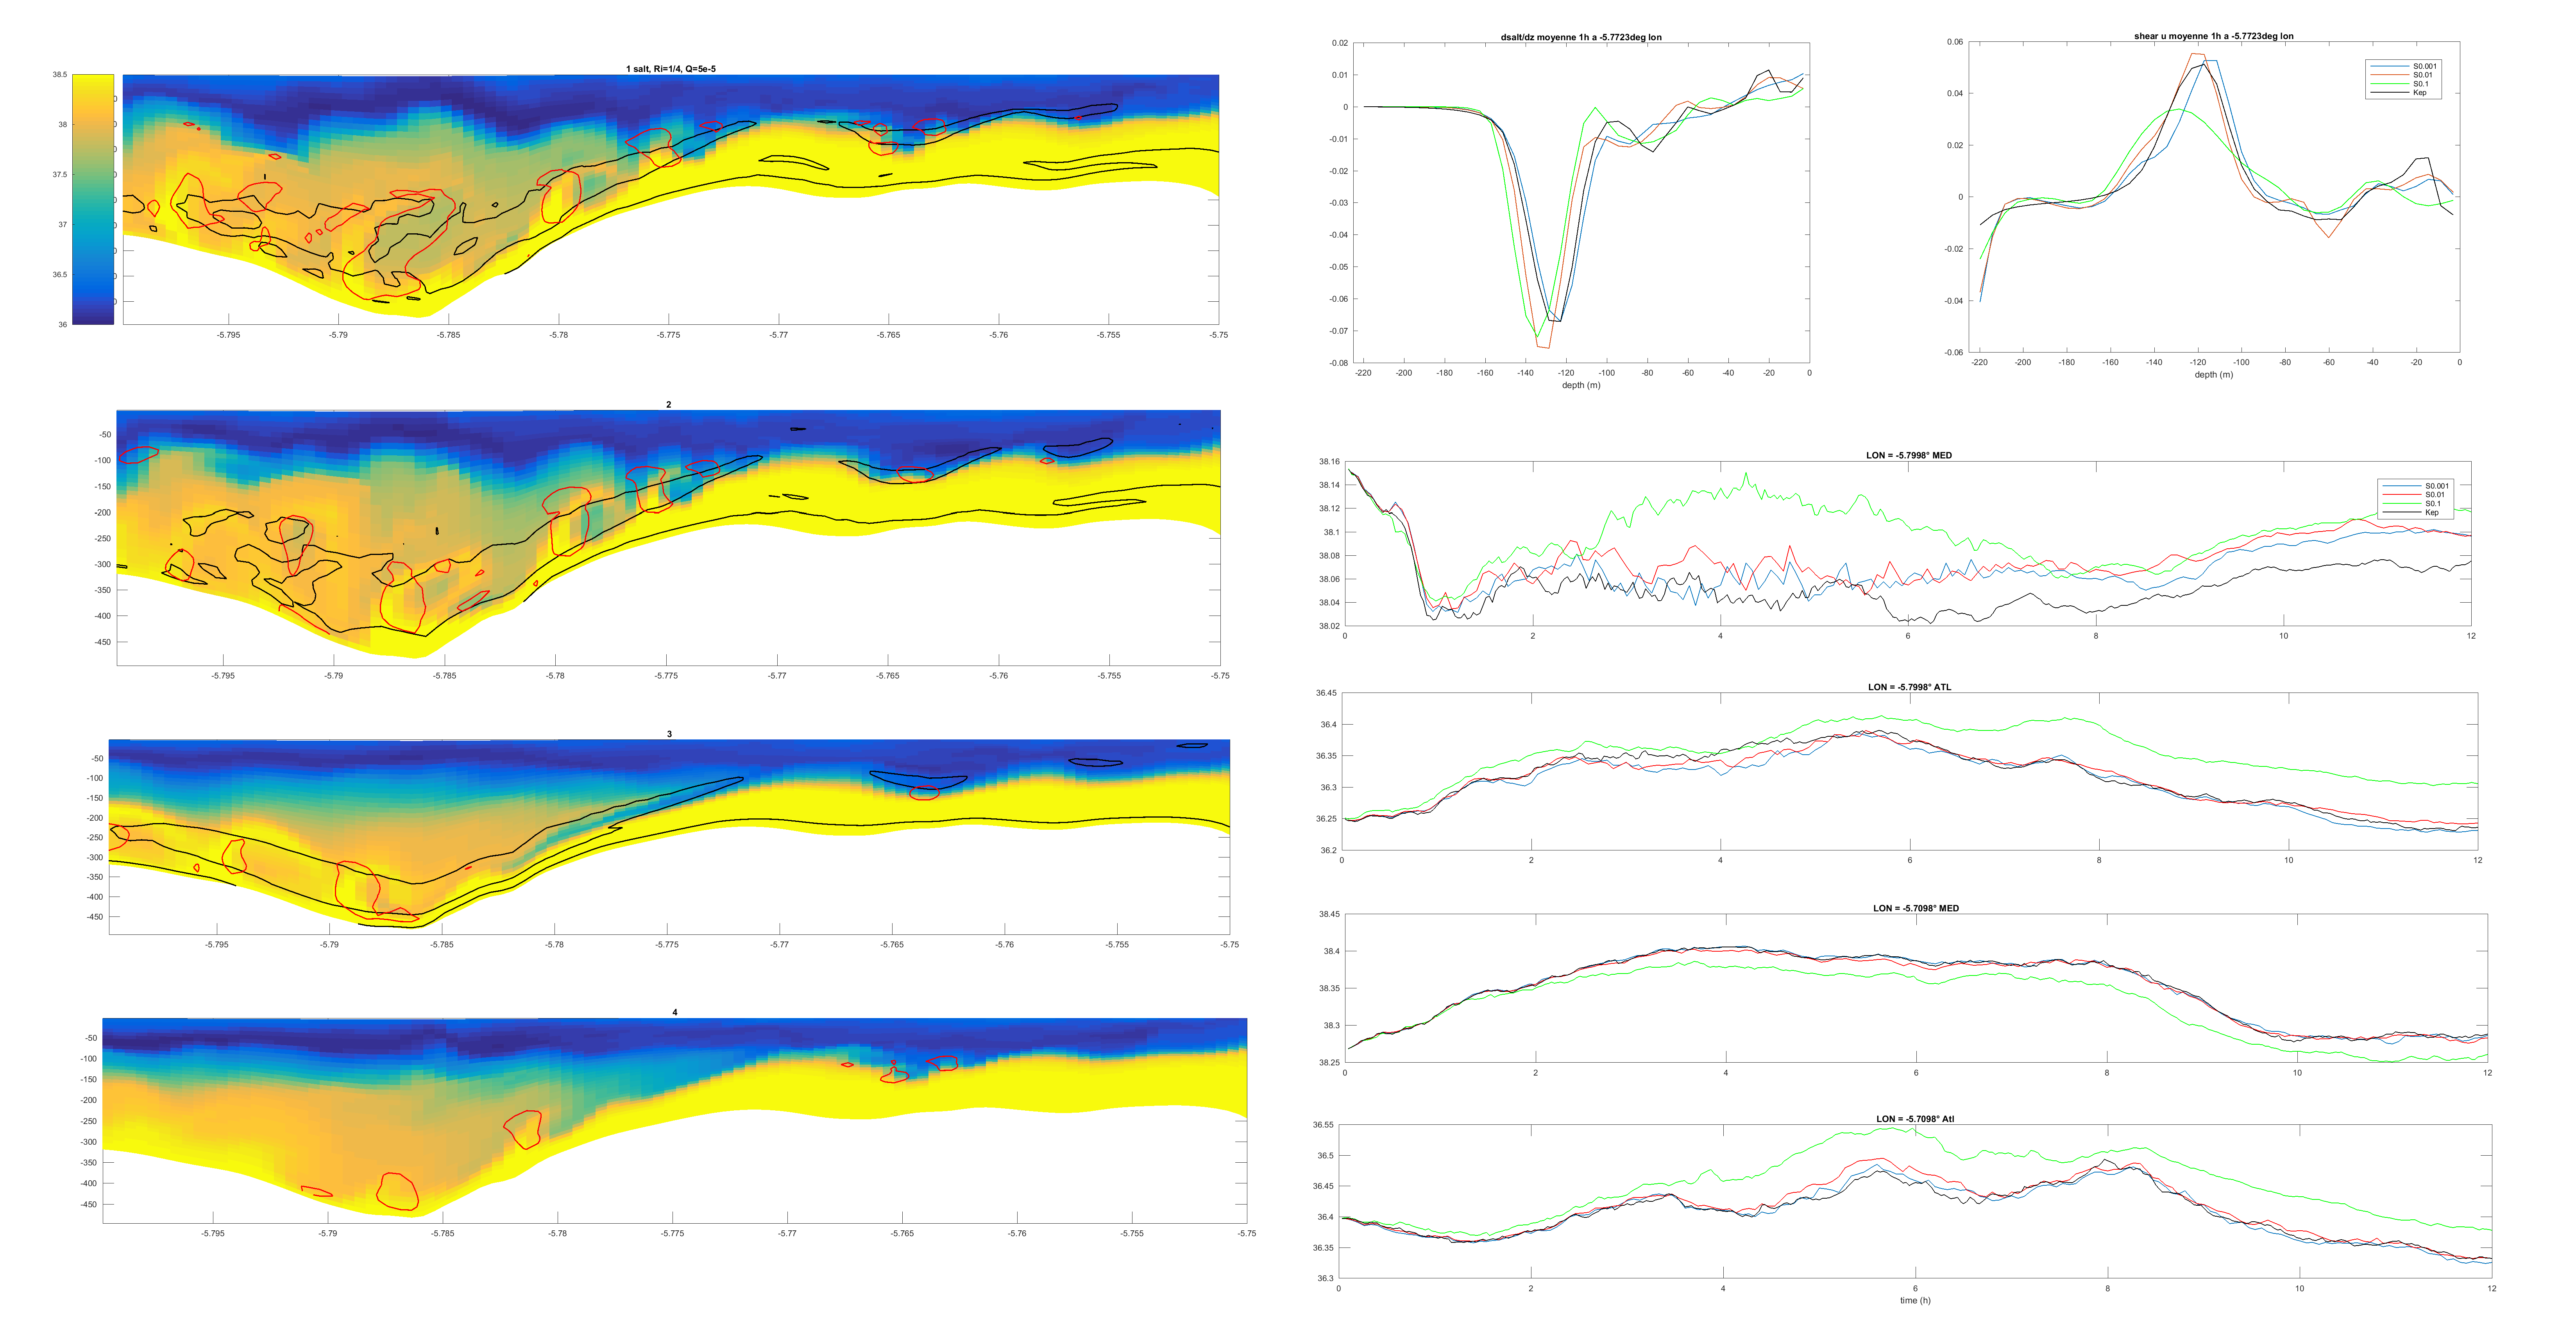
\includegraphics[width=\textwidth]{./GBR3D/Figsmago.png}
 \caption {fiels of salinity at lat = $35.9372^o$ in simu IES at 4h of simulation time  (1:S0.001  2:S0.01  3:S0.1 4:Kep)}
\end{figure}

%-------------------------------------------------------------------------------------
\subsection{Discussion}
Gib :
More mixing expected west of CS than east... Mediterranean vein also mixed in Gulf of Cadiz.

Spatial (here) and temporal variability can be studied... See area of expected billows extends more in south path than northern one. (Millot 20?? : Mixing not the same north or south)



blabla LES..

High resolution modelling of key areas open possibilities in parametrisation, imbricated models etc... tool that needs to be more studied 

The prevalance/importance of numerical dissipation associated with advection scheme needs to be carefully assessed, in particular here the structure of the primary instabilities and how it is resolved/behaves is key at 

Interest for global models but also for field studies as to chose precisely areas. Although need a framework that make comparison of mixing measured across this medium more easy (Gregg review..)



La maquette NH-HR permet, de façon attendue, de raffiner la simulation des ondes solitaires se propageant en direction de la Méditerranée depuis le détroit de Gibraltar. Une étude plus détaillée de ces ondes de grande amplitude à partir d'observations dédiées et, ou, d'une modélisation simultanée avec un modèle simplifié de type KdV devrait fournir de précieuses informations sur l'impact de la résolution sur la dissipation physique et la dissipation numérique, sur la dispersion non-hydrostatique ou encore sur la bonne représentation des processus non-linéaires.\\
La maquette  NH-HR autorise en outre de façon originale la simulation explicite des "grandes structures turbulentes" (simulation dite \textit{LES}) dans la région du détroit de Gibraltar. L'augmentation de la résolution entre les maquettes NH-REF et NH-HR autorise en effet la simulation des structures tourbillonnaires associées aux instabilités primaires de type Kelvin-Helmholtz entre les masses d'eaux méditerranéenne et atlantique. Ces instabilités marquent classiquement l'amorce de la cascade turbulente directe induisant localement un important mélange des masses d'eaux. Ces instabilités ne sont pas représentées dans la simulation NH-REF par manque de résolution effective. Elles ne pourraient être simulées explicitement dans une simulation hydrostatique de même résolution (45 m) dans cette région. Ces instabilités sont en effet associées à une vorticité relative d'axe horizontal qui ne peut être simulée sous une hypothèse hydrostatique. Un résultat important pour cette première simulation pouvant être qualifiée de \textit{LES} concerne les différences importantes entre le mélange simulé au moyen des maquettes NH-REF et NH-HR. L'intercomparaison montre à minima une très forte dépendance au protocole de simulation. La maquette NH-REF (de type \textit{RANS}\footnote{RANS: Reynolds Average Navier Stokes simulation, simulation basée sur une représentation implicite des "grandes structures turbulentes" à partir d'un schéma de fermeture turbulent.}) permet une simulation implicite du mélange et dépend pour cela entièrement du schéma de fermeture turbulente.\\
La maquette NH-HR montre donc l'importance d'une représentation explicite des "grandes structures turbulentes" dans des régions dynamiquement instables telles que la région du ressaut hydraulique. Elle donne de plus l'ordre de grandeur de la résolution horizontale (environ 45 m) et verticale (40 niveaux $\sigma$) permettant la simulation explicite des instabilités primaires.\\
Une première évaluation de la pertinence et de la qualité des structures instables simulées a pu être réalisée à partir d'observations publiées (Wesson and Gregg 1994). Un protocole d'observations dédié devra toutefois être plus spécifiquement mis en oeuvre pour espérer évaluer les caractéristiques principales de ces instabilités (localisation spatio-temporelle, amplitude...) et surtout pour quantifier les caractéristiques statiques du mélange qu'elles induisent. La campagne d'observations planifiée par le SHOM dans la région du détroit à la fin de l'été 2020 (soit un peu plus d'un an après la publication du présent rapport) devrait sans aucun doute répondre à un certain nombre de questions. Les maquettes numériques développées et évaluées dans le cadre du projet Gibraltar 16CR01 pourront être utilisées pour préparer cette campagne via par exemple la génération d'observations synthétiques.\\
Une discussion des principales perspectives associées à l'exploitation de la dynamique simulée d'une part et à l'évolution du protocole de simulation d'autre part est fournie au chapitre \ref{chapitreconclusion}.
%-------------------------------------------------------------------------------------
\section{Campagne de mesure Gibraltar 2020 (en anglais?)}
\subsection{Insights on Campaign Preparation from VHR simulation}
Section ce qui a ete fait pour preparer la campagne

\begin{itemize}
\item déroulé campagne
\item Position mouillages, zones susceptibles d'avoir instas...
\item Propagation des solitons
\item Preparation maquette triple imbrication : choix zoom sur camarinal important (ou non parle que maquette 2 niveaux?)
\end{itemize}


\subsection{Maquette imbriquée, comp quelques obs}




